% ==================================================================
%  HSE Course Project Report — single-file template (fixed)
%  Compile: pdflatex main.tex   (twice)
% ==================================================================
\documentclass[11pt,letterpaper]{article}
\usepackage{fix-cm}
% ---------- Encoding & language (English only) ----------
\usepackage[T1]{fontenc}
\usepackage[utf8]{inputenc}
\usepackage[english]{babel}

% ---------- Geometry (US Letter, uniform 1 inch margins) ----------
\usepackage[
  letterpaper,
  margin=1in,
  headheight=0pt, headsep=0pt, footskip=18pt
]{geometry}

% ---------- Math (must come before the font package) ----------
\usepackage{amsmath}
\usepackage{bm}

% ---------- Fonts (Libertinus serif/sans/mono + matching math) ----------
\usepackage{libertinus}

% ---------- Spacing ----------
\usepackage{setspace}
\setstretch{1.15}

% ---------- Tables & figures ----------
\usepackage{booktabs,array,tabularx,multirow}
\usepackage{graphicx}
\graphicspath{{../figures/}{figures/}{logos/}{../logos/}}
\usepackage{float}
\usepackage{caption}
\captionsetup{font=small,labelfont=bf,skip=4pt}

% ---------- Lists ----------
\usepackage{enumitem}
\setlist{itemsep=2pt,topsep=3pt,parsep=0pt,leftmargin=*}

% ---------- Typography ----------
\usepackage{microtype}

% ---------- Citations (Harvard author–year) ----------
\usepackage[authoryear,round]{natbib}

% ---------- Hyperref (load last) ----------
\usepackage[hidelinks]{hyperref}
\hypersetup{colorlinks=true,linkcolor=black,citecolor=black,urlcolor=blue}

% ---------- Paragraph style ----------
\setlength{\parindent}{1.5em}
\setlength{\parskip}{0.3ex plus 0.1ex minus 0.1ex}

% ---------- Headers / footers ----------
\usepackage{fancyhdr}
\pagestyle{fancy}
\fancyhf{}
\fancyfoot[C]{\small\thepage}
\renewcommand{\headrulewidth}{0pt}
\fancypagestyle{plain}{%
  \fancyhf{}\fancyfoot[C]{\small\thepage}%
  \renewcommand{\headrulewidth}{0pt}}

% ---------- Comments block (one per task, as required) ----------
\newenvironment{taskcomments}[1][Comments]{%
  \par\medskip\noindent
  \begin{quote}\small\textbf{#1.}\enspace\ignorespaces
}{%
  \end{quote}\medskip
}

% ---------- Metadata (edit per assignment) ----------
\usepackage{pgfkeys}
\newcommand{\HSEnumber}{}\newcommand{\HSEtitle}{}
\newcommand{\HSEcourse}{}\newcommand{\HSEprogramme}{Master's Programme}
\newcommand{\HSEstudent}{}\newcommand{\HSEgroup}{}
\newcommand{\HSEsupervisor}{}\newcommand{\HSEdate}{}
\pgfkeys{
  /hse/.is family, /hse,
  number/.store in     = \HSEnumber,
  title/.store in      = \HSEtitle,
  course/.store in     = \HSEcourse,
  programme/.store in  = \HSEprogramme,
  student/.store in    = \HSEstudent,
  group/.store in      = \HSEgroup,
  supervisor/.store in = \HSEsupervisor,
  date/.store in       = \HSEdate,
}
\newcommand{\HSESetup}[1]{\pgfkeys{/hse,#1}}

% ---------- Title page + running header ----------
\renewcommand{\maketitle}{%
  \begin{titlepage}%
    \thispagestyle{empty}\centering
    \vspace*{0.6cm}
    % HSE University Russian emblem and English wordmark
    \raisebox{0.18in}{\includegraphics[width=1.3in]{logos/01_Logo_HSE_full_rus_CMYK.pdf}}%
    \hspace{0.25in}%
    \includegraphics[width=0.44\textwidth]{logos/hse-logo-eng.pdf}\\[0.55cm]
    {\normalsize Faculty of Computer Science\par}
    \vspace{2.2cm}
    \rule{\linewidth}{0.5pt}\\[0.7cm]
    {\LARGE\bfseries \HSEtitle\par}
    \vspace{0.7cm}\rule{\linewidth}{0.5pt}
    \vfill
    {\large\renewcommand{\arraystretch}{1.25}%
     \begin{tabular}{@{}rl@{}}
       \textbf{Course:}     & \HSEcourse \\[0.3em]
       \textbf{Programme:}  & \HSEprogramme \\[0.3em]
       \textbf{Student:}    & \HSEstudent \\[0.3em]
       \textbf{Group:}      & \HSEgroup \\[0.3em]
       \textbf{Supervisor:} & \HSEsupervisor \\
     \end{tabular}\par}
    \vfill{\large \HSEdate\par}\vspace{0.5cm}
  \end{titlepage}%
  \pagenumbering{arabic}%
  \pagestyle{fancy}\fancyhf{}%
  \fancyfoot[C]{\small\thepage}%
  \renewcommand{\headrulewidth}{0pt}%
  \hypersetup{pdftitle={SPARCS: Spotify Pop Association, Regression,
                         Clustering, and SVD -- A Bootstrap-Backed Analysis
                         of Audio Features},
              pdfauthor={\HSEstudent}}%
}

% ==================================================================
\begin{document}
% ==================================================================

\HSESetup{
  number     = {1--5},
  title      = {SPARCS: Spotify Pop Association, Regression, Clustering, and SVD — A Bootstrap-Backed Analysis of Audio Features},
  course     = {Basics of Data Analysis},
  student    = {S M Gazzali Arafat Nishan},
  group      = {Data Science},
  supervisor = {Prof. Boris Grigoryevich Mirkin},
  date       = {Moscow -- 2026},
}

\maketitle

% ------------------------------------------------------------------
\begin{center}
\begin{minipage}{0.9\textwidth}
\small
\textbf{Abstract.}
This report presents the complete set of five homework assignments of the
course \textit{Basics of Data Analysis}, solved on the Spotify Tracks dataset
($\approx$114\,000 rows, 21 variables, 114 genres). Following the supervisor's
advice, all assignments operate on a single homogeneous genre---\textbf{pop},
$n=1\,000$ tracks. \textbf{A1} fits a two-dimensional least-squares regression
of \texttt{loudness} on \texttt{energy}: the fitted line
$\widehat{\mathrm{loudness}} = -13.2765 + 10.4257\cdot\mathrm{energy}$ attains
$\rho = 0.7230$ and a determinacy coefficient $\rho^2 = 0.5228$, with mean
relative absolute errors of 23.13\,\% (data-analysis view) and 20.44\,\%
(machine-learning view); a seeded 80/20 hold-out check confirms that the
pattern generalises (test $R^2 = 0.5101$). \textbf{A2} applies PCA/SVD to five
audio features under range normalization and z-scoring (first two components
retain 67.62\,\% and 65.51\,\% of the scatter, respectively), verifies the
equivalence with conventional correlation-matrix PCA, and derives a 0--100
\emph{hidden ranking factor} of the ``energetic/upbeat'' aspect.
\textbf{A3} runs K-means for $K=4$ and $K=7$ over 15 random initializations
each (best objectives 2496.421 and 1889.485 on standardized data), interprets
both partitions via relative deviations of within-cluster centers from the
grand mean, and judges $K=4$ the better-interpretable partition. \textbf{A4}
builds a contingency table of a self-developed \texttt{popularity level}
feature against the existing \texttt{explicit} flag, computes Quetelet index
and conditional-frequency tables ($\bar q = 0.0371 = \chi^2/n$, $\chi^2 =
37.10$, $p\approx8.8\times10^{-9}$), and determines the minimum sample sizes
for detecting the association at the 95\,\% and 99\,\% levels (162 and 249
observations). \textbf{A5} uses bootstrap (10\,000 resamples) to construct
95\,\% confidence intervals for the mean energy (pivotal $[0.5956,\,0.6173]$,
percentile $[0.5957,\,0.6171]$), to compare two clusters, and to compare the
cluster nearest to the grand mean with it. Every task of every assignment is
followed by an explicit comments section.

\medskip
\textbf{Keywords:} simple linear regression, Pearson correlation, determinacy
coefficient, PCA, SVD, data scatter, hidden factor, K-means, contingency
table, Quetelet index, chi-squared, bootstrap confidence intervals, Spotify
audio features.
\end{minipage}
\end{center}

\newpage
\tableofcontents
\newpage

% ==================================================================
\section{Introduction}\label{sec:intro}

Audio descriptors such as \textit{energy}, \textit{loudness},
\textit{danceability}, and \textit{valence} are widely used to characterise
music, yet their mutual structure is rarely examined with elementary, fully
transparent statistical tools. This project follows the data-analysis (DA)
view of the course \textit{Basics of Data Analysis}
\citep{lecture,lecture3,course}, in which regression, PCA, and K-means are all
treated as \textbf{least-squares approximation problems}: a data matrix is
approximated by a low-complexity model, and the \emph{share of data scatter
explained} measures the quality of the approximation.

The report presents the solutions of Homework Assignments~A1--A5
\citep{course}, all solved on the same dataset:

\begin{center}
\small
\begin{tabular}{@{}llp{8.2cm}@{}}
\toprule
ID & Topic & Core question \\
\midrule
A1 & 2D regression \& correlation & How well does \texttt{energy} linearly
explain \texttt{loudness} within the pop genre, and how precise are the
predictions? \\
A2 & PCA/SVD \& hidden factor & How much of the joint variation of five audio
features is captured by two principal components, how does preprocessing
change the answer, and can a single 0--100 composite score be derived? \\
A3 & K-means clustering & What musically meaningful ``types'' of pop tracks
exist for $K=4$ and $K=7$, and which partition is easier to interpret? \\
A4 & Contingency table & Is the self-developed \texttt{popularity level}
associated with the \texttt{explicit} flag, how strongly, and how many
observations are needed to detect it? \\
A5 & Bootstrap & How uncertain are the mean of \texttt{energy} and the
differences between cluster means? \\
\bottomrule
\end{tabular}
\end{center}

Each assignment section is organised \textbf{task by task}, following the
task lists of the assignment briefs; every task ends with an explicit
\emph{Comments} section reproducing and expanding the commentary of the
corresponding notebook. All calculations are reproducible: each assignment has
its own Jupyter notebook
(\nolinkurl{Assignment1_Correlation_Spotify.ipynb} to
\nolinkurl{Assignment5_Bootstrap_Spotify.ipynb}). The figures in this report
are exported directly from the assignment notebooks, which contain the
complete code. All random procedures use fixed seeds (42 for sampling and
bootstrap, 0--14 for the K-means runs), so every number in this report can be
regenerated exactly.

% ==================================================================
\section{Data and preprocessing}\label{sec:data}

\subsection{The source dataset}\label{sec:rawdata}

The Spotify Tracks dataset \citep{spotify} contains 114\,000 rows and 21
columns spanning 114 genres. Tracks may appear under more than one genre, so
the assignments use the single \texttt{pop} genre as a homogeneous subset,
as described below.

\subsection{The pop subset used in Assignments A1--A5}\label{sec:popsub}

The professor's rule for large datasets is to ``select a smaller subset over a
convenient feature'' \citep{course}. On the advice of the supervisor the study
is restricted to a single homogeneous genre---\textbf{pop}. The A1 notebook
loads the full CSV, filters \texttt{track\_genre} $=$ \texttt{pop}
(\nolinkurl{GENRES} $=$ \texttt{["pop"]}), would down-sample to 1\,000 rows if
the genre were larger, and saves the result as
\texttt{spotify\_pop\_1000.csv}; all later notebooks load this file. The
subset satisfies the course requirements for a dataset---$\ge 80$ objects,
$\ge 5$ features with $\ge 3$ quantitative ones, no missing values---as the
requirement check in the notebook confirms: 1\,000 objects (need $\ge$ 80),
11 features (need $\ge$ 5), 8 quantitative features (need $\ge$ 3):
\texttt{popularity}, \texttt{duration\_ms}, \texttt{danceability},
\texttt{energy}, \texttt{loudness}, \texttt{valence}, \texttt{tempo},
\texttt{acousticness}; 0 missing values (need 0). The nominal feature
\texttt{explicit} (926 non-explicit vs.\ 74 explicit tracks) serves as the
group label. Table~\ref{tab:popdescribe} shows the full \texttt{describe()}
table of the eight quantitative features of the subset.

\begin{table}[H]
\centering
\caption{Summary statistics of the eight quantitative features of the pop
subset ($n=1\,000$).}
\label{tab:popdescribe}
\footnotesize
\setlength{\tabcolsep}{3.5pt}
\begin{tabular}{lrrrrrrrr}
\toprule
 & count & mean & std & min & 25\,\% & 50\,\% & 75\,\% & max \\
\midrule
popularity   & 1000 & 47.576    & 34.040   & 0       & 2       & 66      & 71      & 100 \\
duration\_ms & 1000 & 220672.776 & 56548.741 & 62942  & 183066  & 211522  & 247175.5 & 586075 \\
danceability & 1000 & 0.630     & 0.137    & 0.206   & 0.541   & 0.642   & 0.727   & 0.918 \\
energy       & 1000 & 0.606     & 0.178    & 0.114   & 0.488   & 0.618   & 0.727   & 0.986 \\
loudness     & 1000 & $-6.954$  & 2.563    & $-20.647$ & $-8.600$ & $-6.724$ & $-5.134$ & $-1.100$ \\
valence      & 1000 & 0.506     & 0.212    & 0.038   & 0.344   & 0.498   & 0.678   & 0.969 \\
tempo        & 1000 & 120.927   & 31.066   & 55.832  & 94.999  & 118.660 & 144.028 & 203.983 \\
acousticness & 1000 & 0.344     & 0.286    & 0.000   & 0.083   & 0.281   & 0.576   & 0.983 \\
\bottomrule
\end{tabular}
\end{table}

A check of the track IDs finds 7 repeated \texttt{track\_id}s among the
1\,000 pop rows; all rows are kept as given, and the consequences of this
repetition for statistical inference are discussed in Sections~\ref{sec:a4}
and~\ref{sec:a5}.

% ==================================================================
\section{Assignment A1: two-dimensional regression and correlation}\label{sec:a1}

The analysis follows the approximation (least-squares) perspective of
two-dimensional linear regression and the correlation framework of
Lecture~2 \citep{lecture}, building on the classical treatment of
\citet{galton,pearson}. The notebook follows the seven tasks of the
assignment (slide 44) and uses the lecture formulas
\begin{center}
\small
\begin{tabular}{@{}ll@{}}
\toprule
Quantity & Formula (lecture slides) \\
\midrule
Slope               & $a = \rho\,\sigma(y)/\sigma(x)$ \\
Intercept           & $b = \bar y - a\,\bar x$ \\
Residual variance   & $L(a,b)/N = \sigma^2(y)\,(1-\rho^2)$ \\
Determinacy coefficient & $\rho^2$ \\
DA relative error   & $\mathrm{error}_1 = |y-\hat y|/|y|$ \\
ML relative error   & $\mathrm{error}_2 = |y-\hat y|/|\hat y|$ \\
\bottomrule
\end{tabular}
\end{center}

\subsection{Task 1: find two features with a ``linear-like'' scatterplot}\label{sec:a1t1}

The correlation matrix of the eight quantitative features of the pop subset
was computed and visualised (Figure~\ref{fig:a1corr}), and a scatterplot
matrix of the five candidate features (\texttt{energy},
\texttt{loudness}, \texttt{acousticness}, \texttt{danceability},
\texttt{valence}) with histograms on the diagonal was produced in the
notebook. The five strongest absolute correlations are:
energy--loudness $0.723$; energy--acousticness $-0.649$;
loudness--acousticness $-0.511$; danceability--valence $0.416$;
energy--valence $0.414$.

\begin{figure}[H]
  \centering
  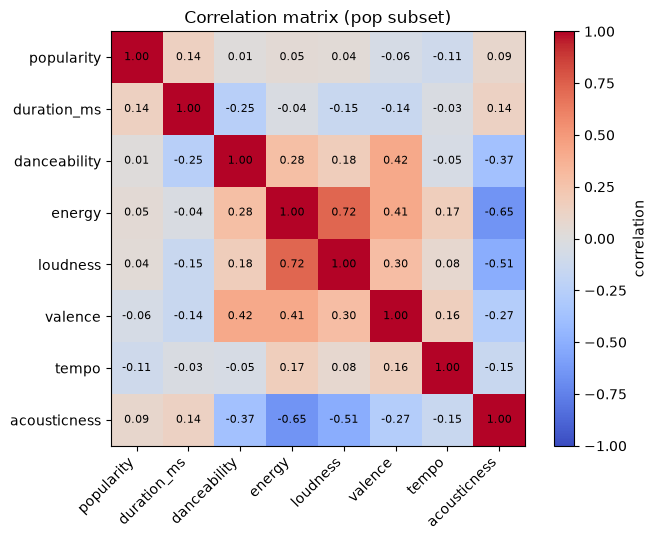
\includegraphics[width=0.62\textwidth]{a1_corr_heatmap_pop1000.png}
  \caption{Correlation matrix of the eight quantitative features of the pop
    subset ($n=1\,000$); \texttt{energy}--\texttt{loudness} (0.72) is the
    strongest positive pair.}
  \label{fig:a1corr}
\end{figure}

\textbf{Choice.} The strongest pair is \textbf{energy} and \textbf{loudness}
($\rho \approx 0.72$). \emph{Energy} (0--1) measures how intense and active a
track feels, and loudness (in dB) is the average volume, so it is natural that
louder tracks feel more energetic. The pair \emph{energy--acousticness} is
also strong ($\rho \approx -0.65$), but its cloud is clearly curved, so
energy--loudness is the better candidate for a linear model. It was retained,
with
\begin{itemize}
  \item predictor $X$: \texttt{energy} (perceptual intensity, scaled on $[0,1]$);
  \item target $Y$: \texttt{loudness} (overall loudness in dB).
\end{itemize}

\begin{taskcomments}[Comments on Task~1]
The correlation matrix alone does not guarantee a ``linear-like'' cloud, so
the scatterplot matrix was inspected as well. The energy--loudness pair is
readily interpretable---energetic tracks tend to be mastered at higher
loudness levels---and satisfies the lecture requirement of a ``more or less
linear-like'' scatter-plot. The runner-up pair (energy--acousticness) has a
comparable correlation but a visibly curved, L-shaped cloud, which would make
a straight-line summary misleading; it is therefore rejected despite its
high correlation.
\end{taskcomments}

\subsection{Task 2: scatterplot and its suitability for linear regression}\label{sec:a1t2}

\begin{figure}[H]
  \centering
  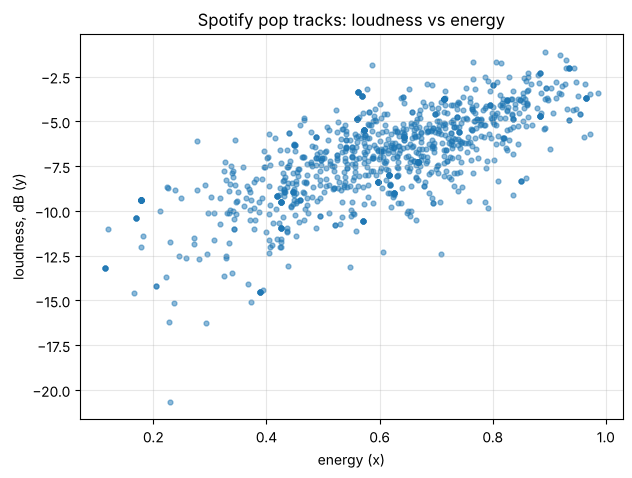
\includegraphics[width=0.55\textwidth]{a1_scatter_pop1000.png}
  \caption{Energy versus loudness for the pop genre ($n=1\,000$).}
  \label{fig:a1scatter}
\end{figure}

The cloud of points in Figure~\ref{fig:a1scatter} rises from the lower-left
(quiet, low-energy tracks) to the upper-right (loud, high-energy tracks),
confirming a positive association. A straight line captures the dominant
trend, yet a residual spread of several decibels remains visible.

\begin{taskcomments}[Comments on Task~2]
A linear model is a reasonable \emph{baseline} (approximation perspective),
but three caveats are visible in the plot. (i) The cloud is \textbf{wide}:
for the same energy, loudness can differ by several dB, so we should not
expect very precise predictions. (ii) There are a few \textbf{quiet outliers}
(5 tracks below $-15$\,dB, all at low energy 0.2--0.4) that pull the left end
of the cloud down, and loudness cannot exceed 0\,dB, so the relation is not
perfectly linear. (iii) The data are one homogeneous group (a single genre),
so there is no risk of Simpson's paradox from mixing groups (slides 26--28).
Overall: \textbf{suitable for a linear regression, with moderate (not high)
precision}. Energy alone cannot determine loudness with high precision;
production style, compression and instrumentation still play important roles.
\end{taskcomments}

\subsection{Task 3: linear regression of loudness over energy}\label{sec:a1t3}

The model is written $\hat{y}_i = a + b x_i$ with the lecture's closed-form
solution (slide 15), equivalent to the closed-form minimisers of the residual
sum of squares $\sum_i e_i^2$. On the pop data,
\begin{align*}
  \bar{x} &= 0.606437, & \bar{y} &= -6.953969, \\
  \sigma(x) &= 0.177632, & \sigma(y) &= 2.561336, \\
  \mathrm{Cov}(X,Y) &= 0.328963, & \rho &= 0.7230.
\end{align*}
Hence
\begin{align*}
  a &= \frac{\mathrm{Cov}(X,Y)}{\sigma^2(x)}
     = \frac{0.328963}{0.177632^2} = 10.425675, &
  b &= -6.953969 - 10.425675 \times 0.606437 = -13.276484.
\end{align*}
The manual computation was checked against \texttt{numpy.polyfit} (the
numerical least-squares line); the two agree to four decimals,
\begin{center}
\small
\begin{tabular}{ll}
\toprule
Manual : & loudness $= 10.4257 \times$ energy $+ (-13.2765)$ \\
\texttt{polyfit} : & loudness $= 10.4257 \times$ energy $+ (-13.2765)$ \\
\bottomrule
\end{tabular}
\end{center}
and the fitted equation is
\begin{equation}
  \boxed{\;\mathrm{loudness} = -13.2765 + 10.4257 \times \mathrm{energy}.\;}
\end{equation}

\begin{figure}[H]
  \centering
  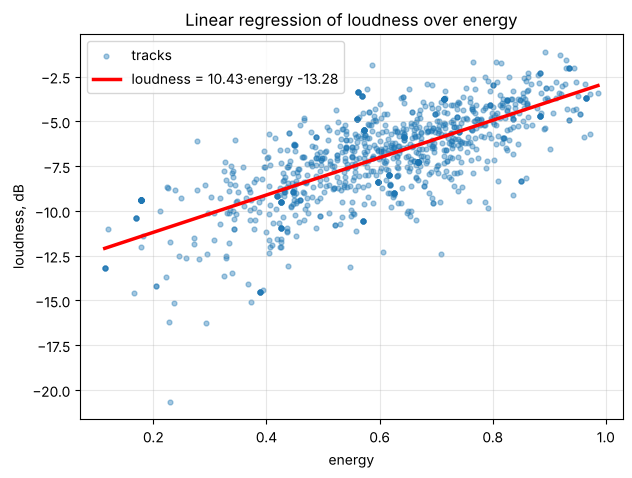
\includegraphics[width=0.55\textwidth]{a1_ols_fit_pop1000.png}
  \caption{The fitted OLS line over the scatter of the 1\,000 pop tracks
    (figure exported from the A1 notebook).}
  \label{fig:a1fit}
\end{figure}

\begin{taskcomments}[Comments on Task~3]
\textbf{Meaning of the slope.} The slope $a \approx 10.43$ is the expected
change in loudness (dB) when energy increases by one full unit (the whole
0$\to$1 scale). Because energy is scaled on the unit interval, a more
practical statement is $\Delta\mathrm{energy}=0.1 \Rightarrow
\Delta\mathrm{loudness}\approx 1.043\,\mathrm{dB}$: a track that is 0.1 more
energetic is expected to be about 1\,dB louder. The slope is positive, as
expected from the scatterplot. \textbf{Meaning of the intercept.} $b \approx
-13.28$\,dB is the expected loudness at energy $=0$. This is an extrapolation
(the lowest energy in the data is about 0.11), so it has no real practical
meaning---as the lecture says, ``this requires some fantasy''. The agreement
of the manual closed-form solution with \texttt{polyfit} confirms the
calculation; the relationship is an observed association, not a causal claim.
\end{taskcomments}

\subsection{Task 4: correlation and determinacy coefficients}\label{sec:a1t4}

The Pearson correlation and the determinacy coefficient are
\begin{equation}
  \rho = \frac{\mathrm{Cov}(X,Y)}{s_X\,s_Y}
       = \frac{0.328963}{0.177632 \times 2.561336} = 0.7230,
  \qquad
  \rho^2 = (0.7230)^2 = 0.5228 \;(52.3\,\%).
\end{equation}
They were verified through the sum-of-squares identity: the variance of $Y$
is $\sigma^2(y) = 6.5604$, the residual variance computed directly is
$L(a,b)/N = 3.1308$, and the lecture identity (slide 15, formula $***$)
\begin{equation}
  \frac{L(a,b)}{N} = \sigma^2(y)\,(1-\rho^2) = 6.5604 \times (1-0.5228) = 3.1308
\end{equation}
holds exactly.

\begin{taskcomments}[Comments on Task~4]
$\rho \approx 0.72$ shows a fairly strong positive linear association. The
\textbf{determinacy coefficient} $\rho^2 \approx 0.52$ is the \emph{proportion
of the variance of loudness explained by the linear regression on energy}:
about 52\,\% of the variability of loudness is accounted for by energy, and
the remaining $\approx 48\,\%$ is residual variance (other factors: genre
style, mastering, instrumentation, etc.). So the relation is real but far
from deterministic; approximately 52\,\% of the observed variation in
loudness is explained, and the residual standard deviation is
$\sqrt{3.1308} = 1.77$\,dB against $\sigma(y) = 2.56$\,dB.
\end{taskcomments}

\subsection{Task 5: predictions for given values of the predictor}\label{sec:a1t5}

Following slide 17, four real tracks with different energy levels were taken
at the 10\,\%, 40\,\%, 70\,\% and 95\,\% quantiles of energy, their loudness
was predicted by the regression, and the predictions were compared with the
observed values (Table~\ref{tab:a1pred}). Table~\ref{tab:a1pure} lists
predictions for convenient energy values (no observed target needed).

\begin{table}[H]
\centering
\caption{Four observed pop tracks at quantiles of energy (row numbers of the
subset in the first column): observed loudness, predicted loudness, and
relative errors (DA: relative to $|y|$; ML: relative to $|\hat y|$).}
\label{tab:a1pred}
\footnotesize
\setlength{\tabcolsep}{5pt}
\begin{tabular}{rlrrrrr}
\toprule
$n$ & Track & Energy & Loudness (dB) & Predicted (dB) & DA error, \% & ML error, \% \\
\midrule
764 & Photograph                    & 0.379 & $-10.480$ & $-9.325$ & 11.02 & 12.38 \\
41  & Ranjha (From ``Shershaah'')   & 0.573 & $-5.843$  & $-7.303$ & 24.98 & 19.99 \\
632 & Ayyayo                        & 0.705 & $-5.525$  & $-5.926$ & 7.27  & 6.77  \\
436 & If You Really Love Me (How Will I Know) & 0.883 & $-4.698$ & $-4.071$ & 13.35 & 15.41 \\
\bottomrule
\end{tabular}
\end{table}

\begin{table}[H]
\centering
\caption{Predicted loudness for four energy values (pure predictions).}
\label{tab:a1pure}
\small
\begin{tabular}{ccccc}
\toprule
Energy $x$ & 0.20 & 0.50 & 0.75 & 0.95 \\
\midrule
Predicted loudness (dB) & $-11.19$ & $-8.06$ & $-5.46$ & $-3.37$ \\
\bottomrule
\end{tabular}
\end{table}

\begin{taskcomments}[Comments on Task~5]
The predictions are in the right range and follow the right order (higher
energy $\to$ louder), but the errors of individual tracks are
\textbf{noticeably large}: from about 7\,\% to 25\,\%. A single track may be
several dB away from the line, because the scatterplot is wide. This is the
point of slides 17--21: a determinacy of $\approx 52\,\%$ does \textbf{not}
guarantee precise individual predictions. The regression is good for
describing the \emph{average} trend, less so for predicting one particular
track. Because the residual standard deviation is approximately 1.77\,dB, an
individual track with the same energy can easily deviate by
$\pm2$--$3$\,dB; the predictions should be regarded as tendencies rather than
exact forecasts.
\end{taskcomments}

\subsection{Task 6: mean relative absolute error on all points, DA vs.\ ML views}\label{sec:a1t6}

Lecture~2 distinguishes two relative-error definitions:
\begin{align}
  \mathrm{error}_1 = \Delta_{\mathrm{DA}}(i) &= \frac{|y_i-\hat{y}_i|}{|y_i|}
    && \text{(data-analysis / descriptive view)}, \\[0.3em]
  \mathrm{error}_2 = \Delta_{\mathrm{ML}}(i) &= \frac{|y_i-\hat{y}_i|}{|\hat{y}_i|}
    && \text{(machine-learning view)}.
\end{align}
Because loudness is negative, absolute values are used in the denominators.
The minimum absolute predicted value is $|\hat{y}|_{\min} = 3.00$\,dB, far
from zero, so the ML view is well defined on these data. Over all 1\,000
tracks:
\begin{align*}
  \mathrm{MRAE}_{\mathrm{DA}} &= 23.13\,\%, & \mathrm{MRAE}_{\mathrm{ML}} &= 20.44\,\%, \\
  \mathrm{median}_{\mathrm{DA}} &= 15.85\,\%, & \mathrm{median}_{\mathrm{ML}} &= 16.19\,\%.
\end{align*}

\begin{figure}[H]
  \centering
  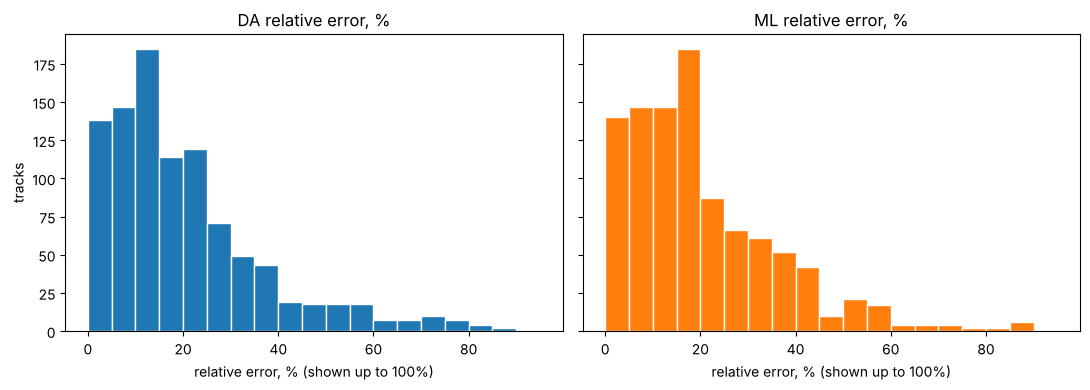
\includegraphics[width=0.85\textwidth]{a1_relative_errors.png}
  \caption{Distributions of the DA (left) and ML (right) relative errors over
    the 1\,000 pop tracks (histogram bins of 5\,\%, shown up to 100\,\%).}
  \label{fig:a1err}
\end{figure}

The counts of extreme cases: \textbf{24 tracks} exceed a DA relative error of
100\,\%, while only \textbf{1 track} exceeds it in the ML view.

\begin{taskcomments}[Comments on Task~6]
The two views give different numbers: DA $\approx 23.1\,\%$ and ML $\approx
20.4\,\%$. The only difference is the denominator: in the DA view it is the
observed value $|y|$, in the ML view the fitted value $|\hat y|$. The
regression line is a \emph{smoothed} version of the data, so for tracks that
are louder than predicted ($|y|<|\hat y|$) the DA error is larger than the ML
error, and for tracks that are quieter than predicted it is the other way
round; on average DA is a bit larger here. The medians are almost equal
(about 16\,\% for both), so the gap is caused by a few extreme cases: the
very loud tracks ($|y| \approx 1$--$2$\,dB) whose predicted loudness is much
lower, where the DA denominator $|y|$ is tiny (24 tracks have a DA error
above 100\,\%, but only 1 has an ML error above 100\,\%), because dividing by
$|\hat{y}|$ damps the errors of quiet tracks. As the lecture says, the two
views ``do differ'' and one should always state which one is used.
\end{taskcomments}

\subsection{Task 7: compare the errors and the determinacy coefficient}\label{sec:a1t7}

The final task juxtaposes the determinacy coefficient with the relative
errors; the notebook prints the full comparison:
\begin{center}
\small
\begin{tabular}{lr}
\toprule
Quantity & Value \\
\midrule
Determinacy $\rho^2$ & 52.3\,\% \\
Unexplained share $100-\rho^2$ & 47.7\,\% \ (share of \textsc{variance}) \\
$\sqrt{1-\rho^2}$ & 69.1\,\% \ (residual s.d.\ relative to $\sigma(y)$) \\
Residual s.d.\ (RMSE) & 1.77\,dB \ vs.\ $\sigma(y) = 2.56$\,dB \\
RMSE relative to mean $|y|$ & 25.4\,\% \\
Mean relative error DA / ML & 23.1\,\% / 20.4\,\% \\
\bottomrule
\end{tabular}
\end{center}

\begin{taskcomments}[Comments on Task~7]
\begin{enumerate}
  \item \textbf{What $\rho^2$ says:} $\rho^2 \approx 52\,\%$ of the variance
        of loudness is explained, so $\approx 48\,\%$ of the variance remains
        unexplained.
  \item \textbf{What the errors say:} the mean relative errors are $\approx
        23\,\%$ (DA) and $\approx 20\,\%$ (ML). These two kinds of numbers are
        \emph{not directly comparable}: 48\,\% is a share of the
        \textbf{variance}, a quadratic quantity, while the relative errors are
        in the units of the data (slides 20--21).
  \item \textbf{Square-root effect:} in the units of the data the typical
        error is $\sqrt{1-\rho^2}\approx 0.69$ of $\sigma(y)$: the residual
        standard deviation is $\approx 1.77$\,dB against $\sigma(y) = 2.56$\,dB.
        So the regression shrinks the typical spread of loudness by only about
        31\,\%, even though it ``explains'' 52\,\% of the variance. Relative
        to the typical size of loudness (mean $|y| \approx 6.95$\,dB), 1.77\,dB
        is $\approx 25\,\%$, which is consistent with the mean relative errors
        of 20--23\,\%.
  \item \textbf{Conclusion for precision:} a determinacy of 52\,\% means a
        typical prediction is off by about $\pm1.8$\,dB, i.e.\ 20--25\,\% of
        the value. A higher $\rho^2$ would give smaller errors; but, as in the
        lecture's Iris example ($\rho^2 = 92.7\,\%$ and still 20--32\,\%
        errors), \textbf{a high determinacy does not by itself warrant high
        precision}.
  \item \textbf{DA vs ML:} 23.1\,\% vs 20.4\,\%---the difference comes from a
        few tracks with very small $|y|$ (very loud), which inflate the DA
        error; the medians are nearly equal ($\approx 16\,\%$). The two views
        would differ much more if $y$ or $\hat y$ were close to 0.
\end{enumerate}
\textbf{Conclusion.} Energy is a meaningful linear predictor of loudness for
pop tracks ($\rho \approx 0.72$, $\rho^2 \approx 0.52$; $+0.1$ energy $\approx
+1$\,dB), but the linear model gives only rough individual predictions
($\approx 20\,\%$ mean relative error).
\end{taskcomments}

\subsection{Residual diagnostic (supplementary check)}\label{sec:a1res}

\begin{figure}[H]
  \centering
  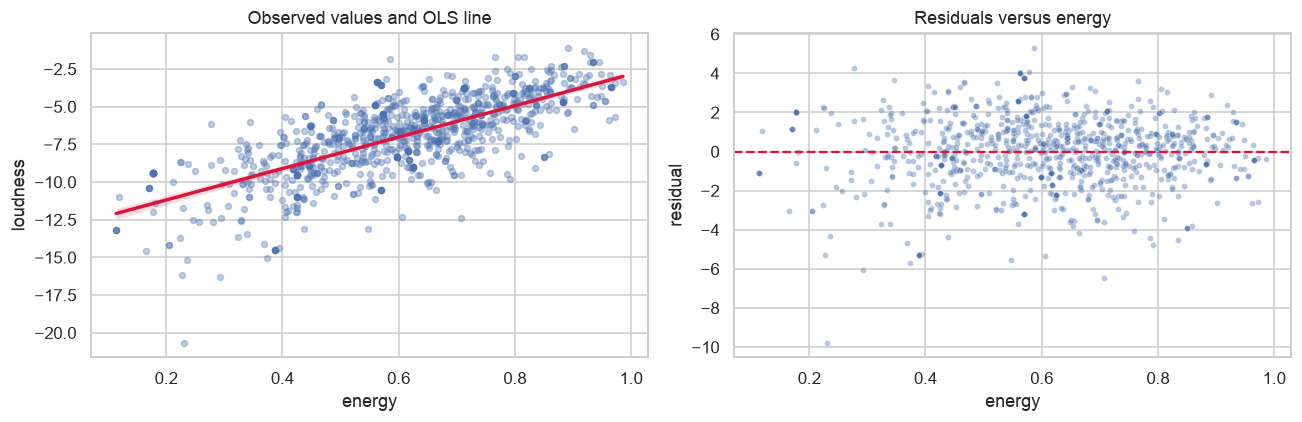
\includegraphics[width=0.95\textwidth]{a1_ols_fit_and_residuals.png}
  \caption{Observed values with the fitted OLS line (left) and residuals
    versus energy (right).}
  \label{fig:a1res}
\end{figure}

The residual-versus-energy plot (right panel of Figure~\ref{fig:a1res}) is
roughly centred on zero and shows no strong systematic curvature, supporting
the linear specification. The vertical spread nevertheless remains
substantial (some residuals exceed $\pm5$\,dB), confirming that energy is only
one of the factors related to loudness. A few low-energy tracks produce large
negative residuals and would merit closer inspection before the model is used
for any high-stakes decision.

% ==================================================================
\section{Assignment A2: PCA/SVD, visualization, and hidden ranking factor}\label{sec:a2}

Following Lecture~3 \citep{lecture3}, PCA is treated as a least-squares
low-rank approximation of a preprocessed data matrix. The assignment consists
of six required parts, A2.1--A2.6, each treated below as a separate task with
its own comments.

\subsection{Task A2.1: feature selection}\label{sec:a2feat}

Five numerical audio features are selected that jointly describe the
\textbf{energetic, upbeat character of the sound}:
\begin{itemize}
  \item \textbf{danceability}: how suitable the track is for dancing (0--1);
  \item \textbf{energy}: perceived intensity and activity of the track (0--1);
  \item \textbf{loudness}: average volume of the track in dB (negative values;
        closer to 0 means louder);
  \item \textbf{valence}: musical positiveness, from sad/dark (0) to
        happy/cheerful (1);
  \item \textbf{tempo}: speed of the track in beats per minute.
\end{itemize}
Together, these features describe a single aspect: the \emph{energetic, upbeat
character of the sound}. The correlation matrix (shown in Task A2.5,
Table~\ref{tab:a2corrmat}) is consistent with this choice: energy, loudness,
valence and danceability are positively related (energy--loudness is 0.72),
and tempo is weakly positive with the other intensity features. The features
have very different scales---tempo is measured in beats per minute (about
55--204), loudness in negative decibels (about $-21$ to $-1$), while the other
three lie on $[0,1]$---so preprocessing is necessary before their
contributions can be compared.

The \texttt{explicit} feature (74 explicit tracks out of 1\,000) is used only
to highlight a group in the visualizations and is excluded from the PCA
calculations; the 74 explicit tracks are designated in advance as the group to
be highlighted in all visualizations.

\begin{taskcomments}[Comments on Task A2.1]
\emph{Acousticness} was deliberately \textbf{not} included: it is the opposite
pole of this aspect (correlation with energy is about $-0.65$), and the hidden
ranking factor in Task A2.6 needs all features pointing in the same
direction. \emph{Popularity}, \emph{duration} and \emph{key} describe other
aspects (success, length, music theory), so they are left out too. Note that
some songs appear more than once in the file (same name and artist listed on
different albums); all 1\,000 rows are kept, as in Assignment~A1. The
selected $1000\times 5$ matrix has no missing values in any of the five
features (checked explicitly in the notebook).
\end{taskcomments}

\subsection{Task A2.2: normalization, SVD, and component contributions}\label{sec:a2svd}

Two preprocessing schemes are applied to the $1000\times5$ matrix $X$:
\begin{align}
  \text{range normalization: } x'_{ij} &= \frac{x_{ij} - \bar{x}_j}
        {\max(x_j) - \min(x_j)}, \\
  \text{z-scoring: } z_{ij} &= \frac{x_{ij} - \bar{x}_j}{\sigma_j},
  \qquad
  \sigma_j = \sqrt{\tfrac{1}{n}\textstyle\sum_i (x_{ij}-\bar x_j)^2},
\end{align}
where the division by $n$ (not $n-1$) matches the calculation used by
scikit-learn's \texttt{StandardScaler}. After range normalization each
feature has mean 0 and range 1 (values may be negative); the method is
sensitive to outliers because the range depends on the minimum and maximum.
After z-scoring each feature has mean 0 and mean square 1.

For each transformed matrix the singular value decomposition $X = U\Sigma V^T$
is computed; the total quadratic data scatter is
$T(X)=\|X\|_F^2=\sum_k \sigma_k^2$, and component $k$ contributes
$\sigma_k^2$, i.e.\ $100\,\sigma_k^2/T(X)$ percent
(Table~\ref{tab:a2svd}). The signs of the singular vectors are fixed so that
the largest absolute weight of each component is positive.

\begin{table}[H]
\centering
\caption{SVD of the pop feature matrix under two preprocessing schemes:
singular values and absolute/percentage contributions to the total scatter.}
\label{tab:a2svd}
\small
\begin{tabular}{lrrrrrr}
\toprule
 & \multicolumn{3}{c}{Range normalization ($T=191.453$)} & \multicolumn{3}{c}{Z-scoring ($T=5000$)} \\
\cmidrule(lr){2-4}\cmidrule(lr){5-7}
PC & $\sigma_k$ & contrib. & \% & $\sigma_k$ & contrib. & \% \\
\midrule
PC1 & 9.212 & 84.865 & 44.33 & 47.040 & 2212.726 & 44.25 \\
PC2 & 6.678 & 44.599 & 23.30 & 32.600 & 1062.753 & 21.26 \\
PC3 & 5.719 & 32.705 & 17.08 & 30.667 & 940.486  & 18.81 \\
PC4 & 4.790 & 22.947 & 11.99 & 22.945 & 526.463  & 10.53 \\
PC5 & 2.517 & 6.337  & 3.31  & 16.049 & 257.572  & 5.15  \\
\midrule
Sum & --- & 191.453 & 100.00 & --- & 5000.000 & 100.00 \\
\bottomrule
\end{tabular}
\end{table}

The right singular vectors $V$ (the feature-to-component direction cosines)
for both normalizations are reported in Tables~\ref{tab:a2vrange}
and~\ref{tab:a2vzscore}; they are the inputs from which the rescaled loadings
of Task A2.4 are computed.

\begin{table}[H]
\centering
\caption{Right singular vectors $V$ after range normalization (total
quadratic scatter $T = 191.452953$).}
\label{tab:a2vrange}
\small
\begin{tabular}{lrrrrr}
\toprule
 & danceability & energy & loudness & valence & tempo \\
\midrule
PC1 &  0.391 &  0.546 &  0.273 &  0.656 &  0.207 \\
PC2 & $-0.406$ &  0.066 &  0.015 & $-0.105$ &  0.905 \\
PC3 & $-0.314$ &  0.660 &  0.434 & $-0.463$ & $-0.251$ \\
PC4 &  0.762 &  0.061 & $-0.011$ & $-0.586$ &  0.269 \\
PC5 &  0.051 & $-0.508$ &  0.858 &  0.020 &  0.048 \\
\bottomrule
\end{tabular}
\end{table}

\begin{table}[H]
\centering
\caption{Right singular vectors $V$ after z-scoring (total quadratic scatter
$T = 5000.000000$, since each standardized feature has mean square 1).}
\label{tab:a2vzscore}
\small
\begin{tabular}{lrrrrr}
\toprule
 & danceability & energy & loudness & valence & tempo \\
\midrule
PC1 &  0.367731 &  0.582532 &  0.525820 &  0.473611 &  0.156960 \\
PC2 & $-0.606840$ &  0.167680 &  0.194586 & $-0.192115$ &  0.727225 \\
PC3 &  0.347237 & $-0.282873$ & $-0.498986$ &  0.432548 &  0.602764 \\
PC4 & $-0.607348$ & $-0.078909$ & $-0.070355$ &  0.737833 & $-0.274871$ \\
PC5 & $-0.084102$ &  0.739118 & $-0.657049$ & $-0.085374$ & $-0.087347$ \\
\bottomrule
\end{tabular}
\end{table}

\begin{taskcomments}[Comments on Task A2.2]
After \textbf{range normalization}, the total quadratic scatter is
191.452953, and the five components account for 44.33\,\%, 23.30\,\%,
17.08\,\%, 11.99\,\% and 3.31\,\% of this scatter (absolute contributions
84.865, 44.599, 32.705, 22.947 and 6.337). After \textbf{z-scoring}, the
total scatter is exactly $5000 = 1000 \times 5$, since each standardized
feature has a mean square of 1; the component contributions are 44.25\,\%,
21.26\,\%, 18.81\,\%, 10.53\,\% and 5.15\,\% (absolute contributions 2212.726,
1062.753, 940.486, 526.463 and 257.572). The absolute contributions of all
components sum to the total scatter in both cases, and the percentages sum to
100\,\%, as the notebook verifies explicitly. The first component alone
carries about 44\,\% under both normalizations, and the first two together
carry about two thirds. The last component is small (3--5\,\%), which means
the five features carry some redundancy: they are not five independent pieces
of information. One caution: these percentages refer to \emph{different
normalized matrices}, so percentages alone do not establish the superiority of
either method.
\end{taskcomments}

\subsection{Task A2.3: two-dimensional projections and the selected group}\label{sec:a2proj}

The ordinary PCA scores are $U\Sigma$ (first two columns); the ``balanced''
factor scale distributes the singular values symmetrically between objects
and features by using $U\sqrt{\Sigma}$ and $V\sqrt{\Sigma}$. The
two-dimensional contribution of the first two components is
\textbf{67.62\,\%} of the scatter under range normalization and
\textbf{65.51\,\%} under z-scoring.

\begin{figure}[H]
  \centering
  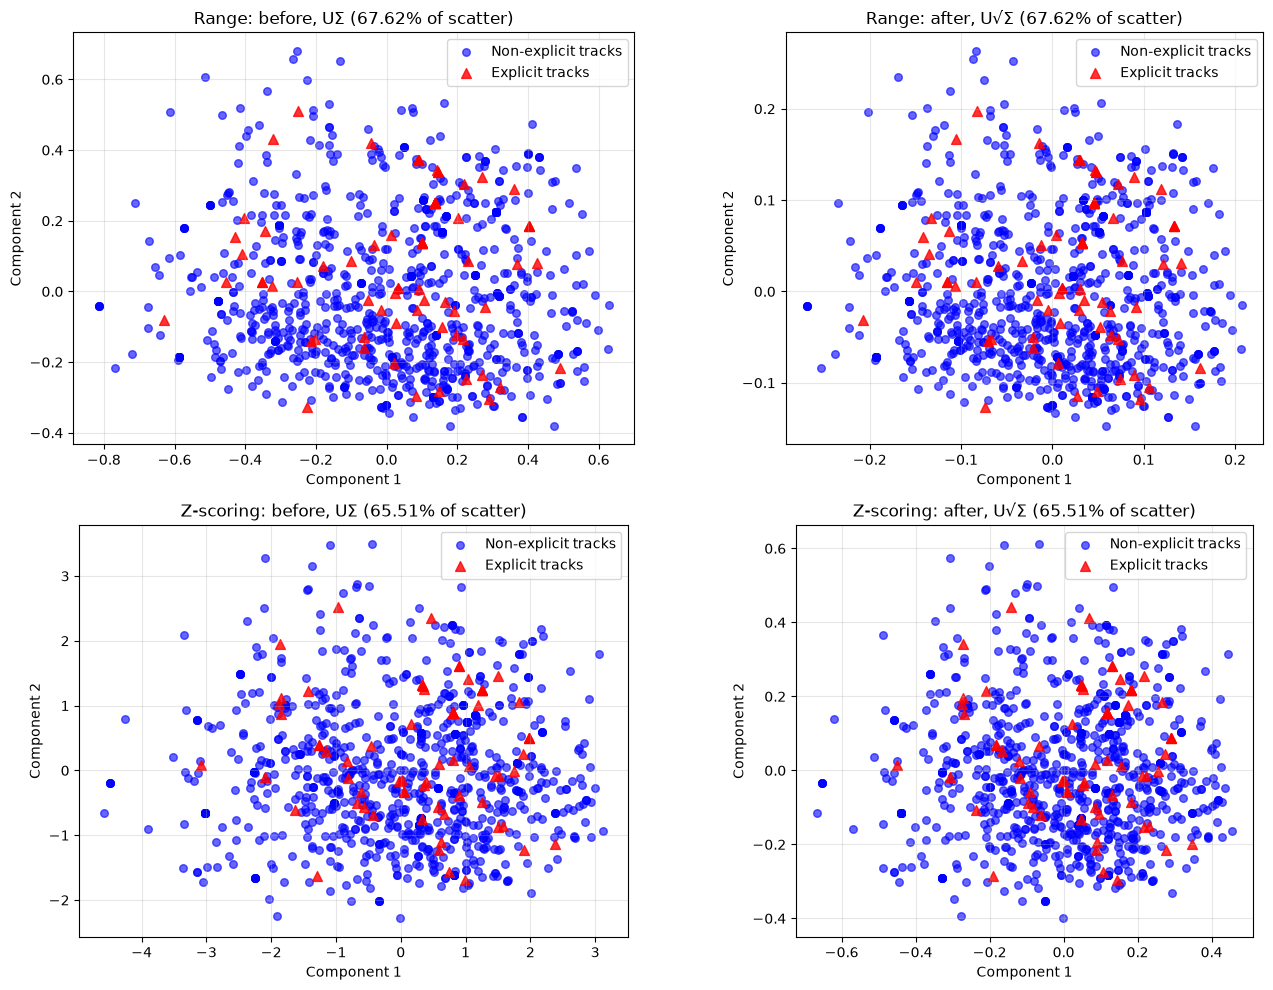
\includegraphics[width=0.98\textwidth]{a2_pca_scores_pop1000.png}
  \caption{First two principal components of the pop tracks under range
    normalization (top) and z-scoring (bottom), before ($U\Sigma$) and after
    rescaling ($U\sqrt{\Sigma}$); red triangles mark the 74 explicit tracks.}
  \label{fig:a2scores}
\end{figure}

The highlighted group is the \textbf{74 explicit tracks} (red triangles).
Under both normalizations the explicit tracks do \emph{not} form a separate
cluster: they are spread over the same area as the non-explicit tracks
(Figure~\ref{fig:a2scores}). They are, however, shifted slightly towards the
upper right: on the z-scored plot the group mean is $(0.36,\,0.32)$ against
$(-0.03,\,-0.03)$ for the other tracks, i.e.\ about 0.24 and 0.31 standard
deviations of the respective components (1.49 and 1.03). With range
normalization the picture is the same ($0.044,\,0.074$ against
$-0.004,\,-0.006$). Explicit tracks in this sample have on average higher
energy (0.65 vs.\ 0.60), higher loudness ($-6.2$ vs.\ $-7.0$\,dB) and a faster
tempo (134 vs.\ 120 bpm), which explains the move towards positive PC1
(energy and loudness) and positive PC2 (tempo).

\begin{taskcomments}[Comments on Task A2.3]
The \texttt{explicit} feature is used only to highlight the group; it is not
in the PCA. The first two components retain 67.62\,\% of the scatter after
range normalization and 65.51\,\% after z-scoring, so about one third of the
information is not visible in these plots---positions and neighbourhoods in
the plane are suggestive, not exhaustive. Rescaling ($U\sqrt{\Sigma}$ instead
of $U\Sigma$) changes the axis scales while preserving the two-component
reconstruction and these contributions. The slightly higher position of the
explicit tracks on the intensity component is a descriptive observation, not
evidence that explicit content \emph{causes} audio-feature changes.
\end{taskcomments}

\subsection{Task A2.4: interpretation of PC1 and PC2 via loadings}\label{sec:a2loadings}

The rescaled loadings $C = V\sqrt{\Sigma}$ of the first two components are
shown in Table~\ref{tab:a2load} and Figure~\ref{fig:a2load} (bar charts of
the z-scored loadings, green for positive and red for negative weights).

\begin{table}[H]
\centering
\caption{Rescaled loadings $C = V\sqrt{\Sigma}$ of the first two components.}
\label{tab:a2load}
\small
\begin{tabular}{lrrrr}
\toprule
 & \multicolumn{2}{c}{Range normalization} & \multicolumn{2}{c}{Z-scoring} \\
\cmidrule(lr){2-3}\cmidrule(lr){4-5}
Feature & PC1 & PC2 & PC1 & PC2 \\
\midrule
danceability & 1.188 & $-1.048$ & 2.522 & $-3.465$ \\
energy       & 1.658 & 0.172   & 3.995 & 0.957   \\
loudness     & 0.829 & 0.039   & 3.606 & 1.111   \\
valence      & 1.992 & $-0.273$ & 3.248 & $-1.097$ \\
tempo        & 0.629 & 2.340   & 1.077 & 4.152   \\
\bottomrule
\end{tabular}
\end{table}

\begin{figure}[H]
  \centering
  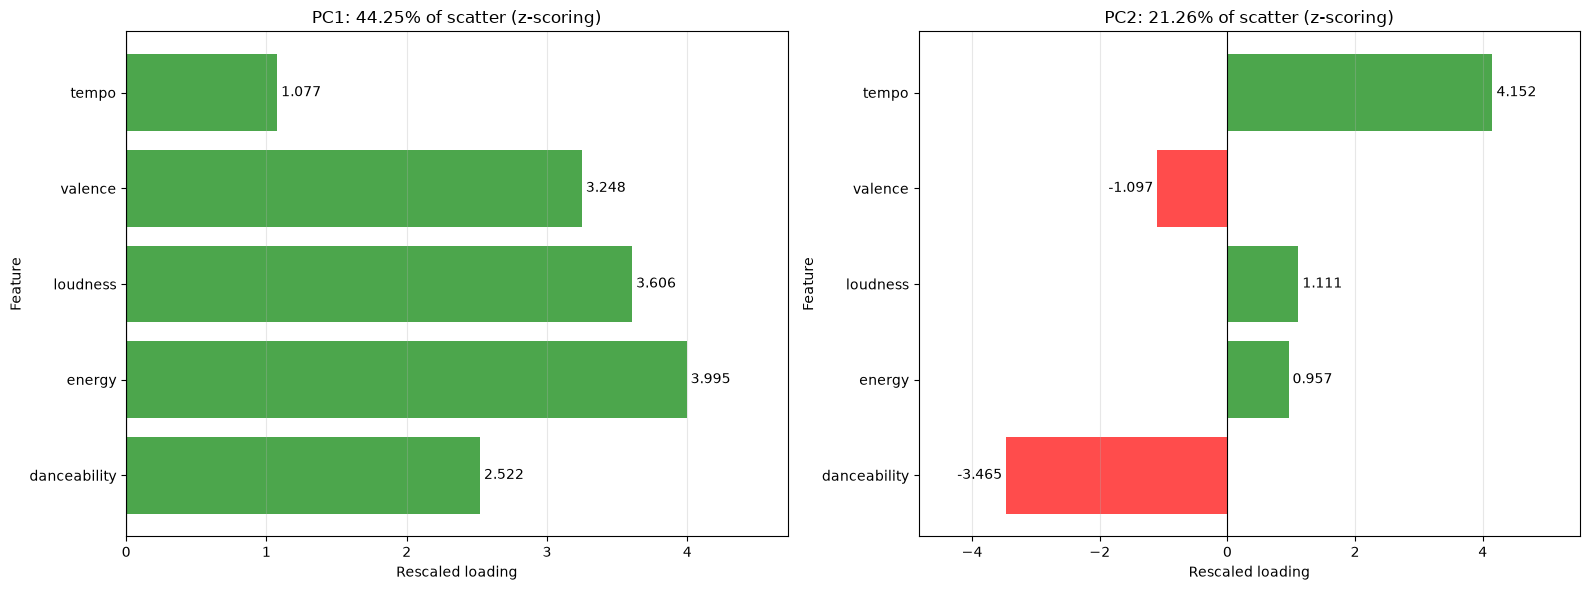
\includegraphics[width=0.98\textwidth]{a2_loadings_pop1000.png}
  \caption{Rescaled loadings of PC1 (44.25\,\% of scatter) and PC2 (21.26\,\%)
    after z-scoring.}
  \label{fig:a2load}
\end{figure}

\textbf{Range normalization.} PC1 is a general ``upbeat and energetic''
component: all loadings are positive---valence (1.992), energy (1.658),
danceability (1.188), loudness (0.829) and tempo (0.629). Tracks with high
PC1 are happier, more energetic and more danceable; loudness has a
surprisingly small weight (see the normalization discussion in Task A2.5).
PC2 mainly reflects tempo: tempo has the dominant loading (2.340), contrasted
with danceability ($-1.048$); energy (0.172), loudness (0.039) and valence
($-0.273$) are close to zero. High PC2 means fast tracks that are less
danceable.

\textbf{Z-scoring.} PC1 is the overall intensity of the sound: energy
(3.995), loudness (3.606), valence (3.248) and danceability (2.522) all have
large positive loadings, tempo a smaller one (1.077). The largest weights are
for energy and loudness, the most strongly correlated pair (0.72). PC2
contrasts tempo (4.152) against danceability ($-3.465$), with valence
slightly negative ($-1.097$) and energy (0.957)/loudness (1.111) mildly
positive: it separates fast, less-danceable (and less cheerful) tracks from
slow, danceable ones. The sign of an entire component is arbitrary; only
relative signs carry the interpretation.

\begin{taskcomments}[Comments on Task A2.4]
Loading magnitudes are compared \textbf{within each component}, never across
components: rescaling preserves the relative weights and signs within each
component. Under range normalization the leading role of energy and valence
on PC1 and the pure tempo contrast on PC2 are easy to name; under z-scoring
the same two-dimensional structure appears with energy/loudness as the PC1
anchors and the tempo-vs-danceability opposition on PC2. These patterns
describe associations in the data, not causal effects.
\end{taskcomments}

\subsection{Task A2.5: conventional PCA and the choice of normalization}\label{sec:a2conv}

The conventional calculation forms the correlation matrix
$B = Y^TY/(n-1)$---equivalently \texttt{np.cov}$(Y^T)\cdot(n-1)/n$, i.e.\
division by $n$---from the z-scored matrix $Y$ and diagonalises it with
\texttt{np.linalg.eigh} (used because the matrix is symmetric and returns
real eigenvalues). The correlation matrix itself is shown in
Table~\ref{tab:a2corrmat}, and the comparison of the three computation routes
in Table~\ref{tab:a2compare}.

\begin{table}[H]
\centering
\caption{Correlation matrix of the five selected features (pop subset,
$n=1\,000$).}
\label{tab:a2corrmat}
\small
\begin{tabular}{lrrrrr}
\toprule
 & dance. & energy & loudness & valence & tempo \\
\midrule
danceability & 1.000 & 0.283 & 0.176 & 0.416 & $-0.055$ \\
energy       & 0.283 & 1.000 & 0.723 & 0.414 & 0.166 \\
loudness     & 0.176 & 0.723 & 1.000 & 0.295 & 0.075 \\
valence      & 0.416 & 0.414 & 0.295 & 1.000 & 0.156 \\
tempo        & $-0.055$ & 0.166 & 0.075 & 0.156 & 1.000 \\
\bottomrule
\end{tabular}
\end{table}

\begin{table}[H]
\centering
\caption{Agreement of the three computation routes on z-scored data: SVD
($\sigma_k^2/n$), the eigenvalues $\lambda_k$ of the correlation matrix, and
\texttt{sklearn} PCA (explained variance $\times\,(n-1)/n$).}
\label{tab:a2compare}
\small
\begin{tabular}{lrrrrr}
\toprule
PC & SVD: $\sigma^2/n$ & Conventional PCA: $\lambda$ & sklearn: var.\ $\times\frac{n-1}{n}$ & SVD, \% & Conventional PCA, \% \\
\midrule
PC1 & 2.212726 & 2.212726 & 2.212726 & 44.254514 & 44.254514 \\
PC2 & 1.062753 & 1.062753 & 1.062753 & 21.255069 & 21.255069 \\
\bottomrule
\end{tabular}
\end{table}

The leading eigenvalues are 2.2127 and 1.0628---exactly $\sigma_k^2/n$ from
the SVD---giving percentage contributions of 44.25\,\% and 21.26\,\%. After
sign alignment (component signs flipped to match the SVD solution), the
balanced factors obtained through SVD and through the correlation matrix
coincide within numerical precision (differences of order $10^{-15}$), and the
scores coincide with \texttt{sklearn} PCA to order $10^{-14}$
(Figure~\ref{fig:a2conv}). For z-scored data, SVD and the eigen-decomposition
of the correlation matrix are two ways of computing the same thing.

\begin{figure}[H]
  \centering
  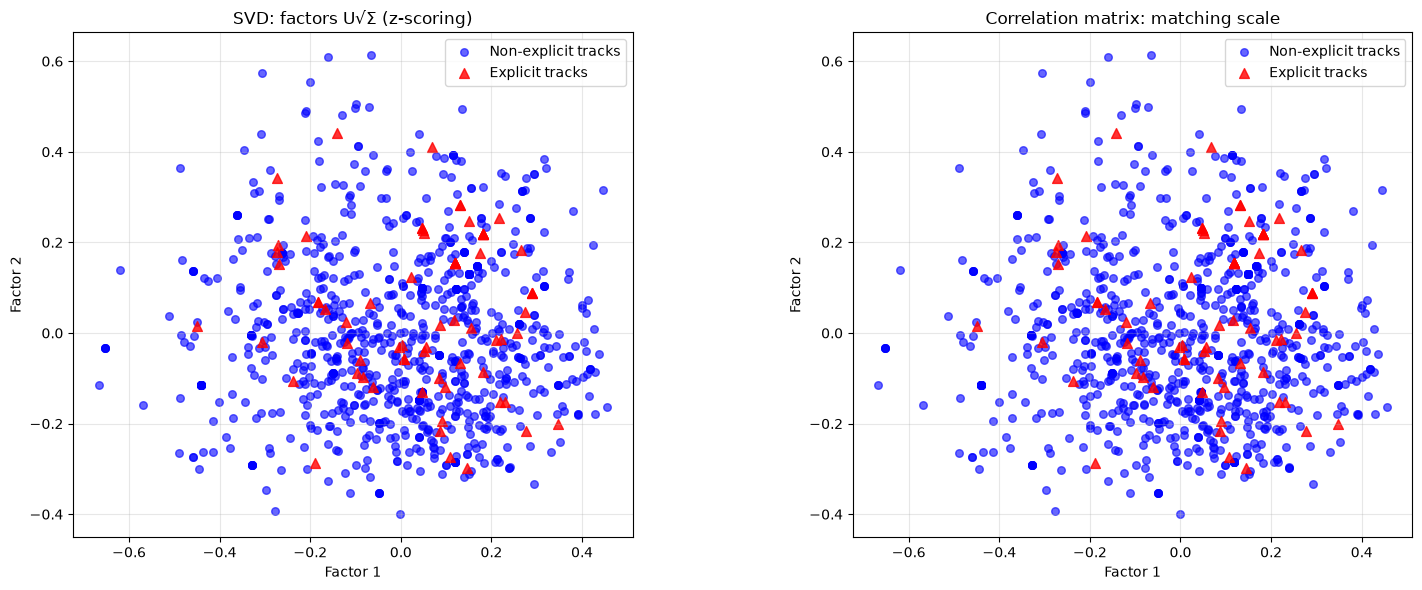
\includegraphics[width=0.95\textwidth]{a2_conventional_pca_pop1000.png}
  \caption{Balanced factors $U\sqrt{\Sigma}$ from SVD on z-scored data (left)
    and the matching factors from the eigendecomposition of the correlation
    matrix (right); the two solutions coincide within numerical precision.}
  \label{fig:a2conv}
\end{figure}

\textbf{Choice of normalization: z-scoring}, for three reasons.
\begin{enumerate}
  \item \textbf{Range normalization depends on extreme values.} Loudness has
        a few very quiet tracks (the minimum is $-20.6$\,dB), which stretch
        its range to 19.5\,dB, about 7.6 standard deviations; the other
        features have ranges of only 4.4--5.2 standard deviations. As a
        result, loudness contributes only \textbf{8.97\,\%} of the
        range-normalized scatter, whereas valence contributes 27.13\,\%,
        tempo 22.94\,\%, energy 21.67\,\% and danceability 19.29\,\%. A
        handful of outliers therefore reduce the weight of a whole feature.
        This is why loudness has such a small loading on PC1 under range
        normalization, although it is strongly related to energy.
  \item \textbf{Z-scoring treats all features equally.} Each standardized
        feature has a variance of 1 and contributes exactly 20\,\% of the
        scatter, so the components reflect the correlation structure rather
        than the accidental extreme values. Under z-scoring PC1 correctly
        shows energy and loudness as the leading, strongly related features.
  \item \textbf{The 2D contribution does not decide.} The first two components
        retain 67.62\,\% (range) and 65.51\,\% (z-scoring) of their own
        tables' scatter; this small difference is partly due to the
        under-weighted loudness, and cannot be used alone to say that range
        normalization is better.
\end{enumerate}

\begin{taskcomments}[Comments on Task A2.5]
Range normalization could be preferred when outliers are absent and the
original ratios between feature spreads are meaningful; it is not the case
here. Neither preprocessing is universally best, but z-scoring expresses
``equal average importance of standardized features'', which matches the goal
of comparing audio features measured in incommensurable units (dB, bpm,
dimensionless scores). The numerical proof of equivalence (Table~\ref{tab:a2compare} and
Figure~\ref{fig:a2conv}, with differences of order $10^{-14}$)
confirms that the ``preprocessing + SVD'' pipeline is not an approximation
\emph{to} PCA but \emph{is} PCA.
\end{taskcomments}

\subsection{Task A2.6: hidden ranking factor on a 0--100 scale}\label{sec:a2hidden}

Each of the five features is rescaled to a 0--100 percentile-style range,
\begin{equation*}
  x^{\mathrm{rank}}_{ij}
  = 100\,\frac{x_{ij}-\min_i x_{ij}}{\max_i x_{ij}-\min_i x_{ij}},
\end{equation*}
and the first right singular vector of the \emph{uncentered} ranked
matrix is computed, oriented to have positive weights (\texttt{Vt[0].sum() >
0}). The resulting weights are
\begin{center}
\small
\begin{tabular}{lccccc}
\toprule
Feature & loudness & danceability & energy & valence & tempo \\
\midrule
Weight & 0.542 & 0.468 & 0.452 & 0.406 & 0.344 \\
\bottomrule
\end{tabular}
\end{center}
The first factor explains \textbf{93.46\,\%} of the uncentered
ranking-normalized scatter about zero, and the raw factor scores are finally
rescaled so that the minimum observed composite equals 0 and the maximum
equals 100 (the calibration anchor; a component score's scale is otherwise
arbitrary). Table~\ref{tab:a2ranktop} shows the first ten observations with
their ranked features and factor scores.

\begin{table}[H]
\centering
\caption{Features and hidden factor on a 0--100 scale: the first ten rows of
the ranked table.}
\label{tab:a2ranktop}
\footnotesize
\setlength{\tabcolsep}{4.5pt}
\begin{tabular}{rlrrrrrrl}
\toprule
$n$ & Track & dance. & energy & loudness & valence & tempo & Factor & Explicit \\
\midrule
0 & Blinding Lights       & 43.26 & 70.64 & 75.27 & 31.77 & 77.74 & 62.87 & no \\
1 & Mann Mera             & 46.21 & 74.66 & 65.41 & 35.96 & 91.79 & 66.04 & no \\
2 & Summer High           & 91.85 & 48.97 & 72.32 & 98.17 & 39.93 & 81.16 & no \\
3 & Under The Influence   & 74.02 & 66.06 & 77.34 & 29.19 & 41.28 & 62.77 & yes \\
4 & Starboy               & 66.43 & 54.24 & 69.74 & 48.10 & 87.86 & 70.49 & yes \\
5 & Insane                & 82.87 & 52.52 & 69.66 & 28.55 & 29.12 & 55.11 & no \\
6 & Akhiyaan              & 72.75 & 57.80 & 59.55 &  3.22 & 29.83 & 42.19 & no \\
7 & Daku                  & 90.03 & 50.92 & 75.67 & 49.07 & 28.50 & 65.24 & no \\
8 & Jhoom - R\&B Mix      & 64.04 & 32.80 & 48.33 & 62.18 & 16.29 & 40.61 & no \\
9 & Na Ja                 & 79.49 & 61.35 & 72.83 & 84.42 & 23.11 & 73.01 & no \\
\bottomrule
\end{tabular}
\end{table}

The five lowest- and highest-scoring observations (unique track names) are
listed in Table~\ref{tab:a2rankends}.

\begin{table}[H]
\centering
\caption{Five observations with the lowest and five with the highest hidden
factor scores (unique track names; ranked features on the 0--100 scale).}
\label{tab:a2rankends}
\footnotesize
\setlength{\tabcolsep}{4.5pt}
\begin{tabular}{rlrrrrrrl}
\toprule
 & Track & dance. & energy & loudness & valence & tempo & Factor & Explicit \\
\midrule
\multicolumn{9}{l}{\textit{Lowest five}} \\
887 & Blue Banisters            & 23.46 &  0.00 & 38.25 & 14.37 & 23.70 &  0.00 & no \\
875 & Happiness is a butterfly  & 36.66 &  0.57 & 49.40 & 12.65 &  9.90 &  5.09 & no \\
767 & Mujhe Peene Do            &  8.71 & 25.23 & 60.21 & 14.69 &  0.00 &  6.08 & no \\
684 & TV                        & 28.93 & 13.99 & 28.08 &  8.67 & 56.96 &  9.04 & no \\
968 & Zara Zara - MTV Unwind    & 53.65 & 13.30 &  0.00 & 26.61 & 54.10 & 10.72 & no \\
\midrule
\multicolumn{9}{l}{\textit{Highest five}} \\
426 & Bad Boy (feat.\ Luana Kiara) & 61.52 & 89.22 & 100.00 & 78.30 & 83.84 & 100.00 & no \\
680 & Expert Jatt                & 78.51 & 95.64 & 91.22 & 65.40 & 78.44 & 99.28 & no \\
656 & Libaas                     & 82.58 & 73.28 & 89.71 & 93.23 & 70.29 & 98.89 & no \\
530 & Thaar Maar Thakkar Maar    & 81.04 & 94.95 & 83.27 & 93.45 & 51.43 & 98.30 & no \\
192 & There's Nothing Holdin' Me Back & 92.70 & 80.16 & 84.84 & 100.00 & 44.66 & 98.27 & no \\
\bottomrule
\end{tabular}
\end{table}

By group, the 74 explicit tracks average \textbf{64.27} (median 70.29, range
13.48--89.75) against \textbf{58.31} (median 60.39, range 0--100) for the 926
non-explicit tracks (Figure~\ref{fig:a2hidden}): the explicit group sits
noticeably higher on the hidden ``energetic/upbeat'' scale.

\begin{figure}[H]
  \centering
  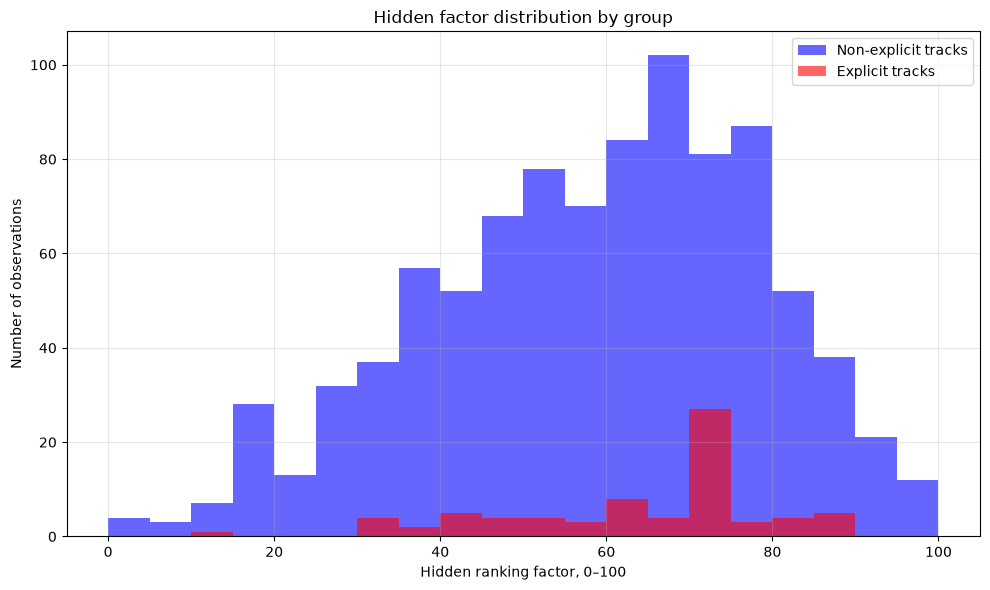
\includegraphics[width=0.62\textwidth]{a2_hidden_factor_hist.png}
  \caption{Distribution of the hidden ranking factor (0--100) for
    non-explicit and explicit tracks.}
  \label{fig:a2hidden}
\end{figure}

\begin{taskcomments}[Comments on Task A2.6]
All weights are positive, so a higher score means a higher overall level of
the features---a \textbf{louder, more energetic, more danceable, more cheerful
and faster track}. The hidden factor can be read as the \emph{overall
energetic/upbeat intensity} of the sound, with loudness, danceability and
energy contributing most. The 93.46\,\% share is high because all
ranking-normalized values are non-negative, so the leading uncentered
component largely captures the common level of the features; it uses a
different transformation and reference point from those in Tasks A2.2--A2.3,
so it should not be compared with the percentages there. The mean score is
64.27 for explicit tracks and 58.31 for non-explicit tracks (medians 70.29
and 60.39): a descriptive group difference---explicit tracks tend to sound
more intense---while the groups overlap strongly (explicit tracks range from
13.48 to 89.75). The endpoints 0 and 100 correspond to the observations with
the lowest and highest factor values in this sample: the lowest score belongs
to \emph{Blue Banisters} (it has the lowest energy of all tracks, and low
valence and danceability) and the highest to \emph{Bad Boy (feat.\ Luana
Kiara)} (the loudest track, with high energy and valence). Note that some
songs appear several times in the file (for instance, \emph{Blue Banisters}
is listed four times with identical features), so the lowest/highest lists
show unique track names. The score is a composite measure of the selected
features relative to this sample, not a validated measure of musical quality.
\end{taskcomments}

% ==================================================================
\section{Assignment A3: K-means clustering}\label{sec:a3}

The assignment brief asks to (1) choose 3 or more quantitative features,
explain the choice and apply K-means for $K=4$ and $K=7$, with about 10--15
runs from random initializations recorded and the best run chosen by the
criterion value; (2) interpret each of the two chosen partitions with the
help of relative differences between within-cluster centers and the grand
mean; (3) make a judgement on which partition is better for interpretation.

\subsection{Task 1: features, standardization, and fifteen random initializations}\label{sec:a3t1}

\paragraph{Feature selection.}
Five quantitative features describe the \textbf{musical character and mood}
of a pop track:
\begin{itemize}
  \item \textbf{danceability} --- how suitable the track is for dancing (0--1);
  \item \textbf{energy} --- perceived intensity and activity (0--1);
  \item \textbf{valence} --- musical positiveness, from sad/dark (0) to
        happy/cheerful (1);
  \item \textbf{acousticness} --- confidence that the track is acoustic
        rather than electronic (0--1);
  \item \textbf{tempo} --- speed of the track in beats per minute.
\end{itemize}
These features describe how a track \emph{sounds}, so clusters of tracks with
similar values can be read as musical ``types'' (mellow acoustic tracks, fast
upbeat tracks, danceable happy tracks, etc.). All five are non-negative, so
relative deviations of cluster means from the grand mean (in per cent) are
meaningful for each of them.

\paragraph{Standardization.}
Before clustering, the features are standardized,
$z_{ij} = (x_{ij}-\bar{x}_j)/\sigma_j$ (division by $n$, matching
\texttt{StandardScaler}), because K-means minimises Euclidean distances and,
without normalization, tempo (about 55--204 bpm) would dominate the
objective. The overall means in original units are danceability 0.630, energy
0.606, valence 0.506, acousticness 0.344, and tempo 120.927 bpm.

\paragraph{The algorithm and the runs.}
K-means \citep{macqueen} alternates between assigning observations to the
nearest centre and updating each centre to the mean of its cluster; the
objective is the within-cluster sum of squared Euclidean distances on
standardized data,
\begin{equation}
  J = \sum_{c=1}^{K}\sum_{i\in C_c} \lVert z_i - \mu_c \rVert^2 .
\end{equation}
For each $K\in\{4,7\}$ the algorithm is run 15 times with different random
initializations (\texttt{init='random'}, \texttt{n\_init=1},
\texttt{max\_iter=300}, \texttt{algorithm='lloyd'}, one seed per run
0--14); the recorded objectives and iteration counts are shown in
Table~\ref{tab:a3runs} and Figure~\ref{fig:a3runs}.

\begin{table}[H]
\centering
\caption{Within-cluster objective $J$ over 15 random initializations (the
same seed is used for both $K$).}
\label{tab:a3runs}
\small
\begin{tabular}{rrr}
\toprule
Seed & $K=4$ & $K=7$ \\
\midrule
0  & 2501.079 & 1921.298 \\
1  & 2501.683 & 1904.235 \\
2  & 2502.458 & 1906.379 \\
3  & \textbf{2496.421} & 1892.807 \\
4  & 2497.376 & 2023.827 \\
5  & 2512.519 & 1973.778 \\
6  & 2511.983 & 1914.467 \\
7  & 2512.927 & 1892.373 \\
8  & 2555.671 & 1909.000 \\
9  & 2501.601 & 1999.777 \\
10 & 2555.684 & 1904.216 \\
11 & 2512.924 & 1923.040 \\
12 & 2512.829 & 1920.238 \\
13 & 2512.040 & 1944.670 \\
14 & 2570.481 & \textbf{1889.485} \\
\bottomrule
\end{tabular}
\end{table}

\begin{figure}[H]
  \centering
  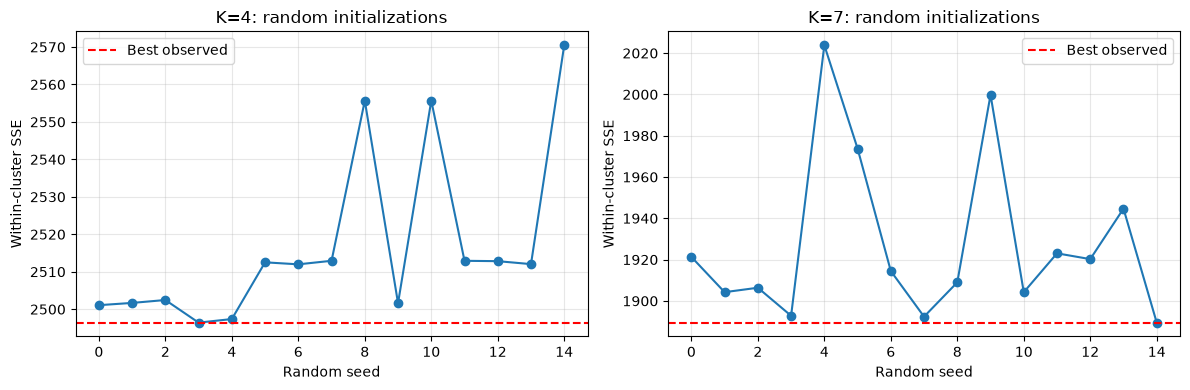
\includegraphics[width=0.98\textwidth]{a3_kmeans_runs.png}
  \caption{Objective values of the 15 random initializations for $K=4$ (left)
    and $K=7$ (right); the dashed line marks the best observed run.}
  \label{fig:a3runs}
\end{figure}

For $K=4$, the lowest objective is obtained with seed~3: $J = 2496.421$
(16 iterations). For $K=7$, the best run uses seed~14 with $J = 1889.485$
(16 iterations). The selected runs are exactly these two; both needed 16
iterations to converge.

\begin{taskcomments}[Comments on Task~1]
For $K=4$, the 15 runs fall into three groups of local optima: six runs at
about 2496--2503 (seeds 0, 1, 2, 3, 4, 9), six at about 2512 (seeds 5, 6, 7,
11, 12, 13), and three at about 2556--2570 (seeds 8, 10, 14); six runs end
within 0.25\,\% of the best value, so the solution is fairly stable. For
$K=7$, the values are more scattered (1889.485 to 2023.827, a spread of about
7\,\%), and only seeds 14, 7 (1892.373) and 3 (1892.807) are within 0.2\,\%
of the best; with more clusters there are more local optima, so the choice of
the best of several runs matters more. The standardized data scatter is 5000
(1000 observations $\times$ 5 features), so the selected partitions explain
about \textbf{50.1\,\%} ($1 - 2496.421/5000$) and \textbf{62.2\,\%} ($1 -
1889.485/5000$) of it. The objective for $K=7$ is about 24.3\,\% lower than
for $K=4$, but a lower objective for $K=7$ alone does not establish a better
partition: increasing the number of clusters always reduces within-cluster
scatter, and interpretability also matters. Finally, the ``best'' runs are
the best \emph{observed} among 15, not a proof of the global optimum.
\end{taskcomments}

\subsection{Task 2: interpretation of the chosen partitions}\label{sec:a3t2}

Each partition is interpreted through the relative differences between
within-cluster centres and the grand mean \emph{in the original units},
\begin{equation}
  d_{cj} = 100\,\frac{\bar{x}_{cj} - \bar{x}_j}{\bar{x}_j}.
\end{equation}
The overall means are danceability 0.630, energy 0.606, valence 0.506,
acousticness 0.344, and tempo 120.9 bpm. Clusters are numbered by increasing
mean energy. Tables~\ref{tab:a3k4} and~\ref{tab:a3k7} report the cluster
means, sizes and deviations; Figures~\ref{fig:a3prof} and the named
interpretations follow.

\begin{table}[H]
\centering
\caption{K-means with $K=4$ (best run, seed~3): cluster means in original
units, sizes, and relative deviations from the grand mean (\%).}
\label{tab:a3k4}
\small
\begin{tabular}{crrrrrrr}
\toprule
 & \multicolumn{5}{c}{Cluster mean} & & \\
\cmidrule(lr){2-6}
Cluster & dance. & energy & valence & acoustic. & tempo & Size & Share, \% \\
\midrule
1 & 0.52 & 0.40 & 0.34 & 0.71 & 111.60 & 253 & 25.3 \\
2 & 0.63 & 0.65 & 0.37 & 0.21 & 102.51 & 235 & 23.5 \\
3 & 0.61 & 0.66 & 0.60 & 0.27 & 162.35 & 241 & 24.1 \\
4 & 0.75 & 0.72 & 0.70 & 0.18 & 108.77 & 271 & 27.1 \\
\midrule
\multicolumn{8}{l}{\textit{Relative deviations $d_{cj}$, \%}} \\
1 & $-17.3$ & $-34.1$ & $-33.5$ & $+106.2$ & $-7.7$  & & \\
2 & $+0.6$   & $+7.6$   & $-26.1$ & $-38.3$  & $-15.2$ & & \\
3 & $-3.4$   & $+8.3$   & $+18.4$ & $-20.6$  & $+34.3$ & & \\
4 & $+18.6$  & $+17.9$  & $+37.5$ & $-47.5$  & $-10.1$ & & \\
\bottomrule
\end{tabular}
\end{table}

\begin{table}[H]
\centering
\caption{K-means with $K=7$ (best run, seed~14): cluster means in original
units, sizes, and relative deviations from the grand mean (\%).}
\label{tab:a3k7}
\small
\begin{tabular}{crrrrrrr}
\toprule
 & \multicolumn{5}{c}{Cluster mean} & & \\
\cmidrule(lr){2-6}
Cluster & dance. & energy & valence & acoustic. & tempo & Size & Share, \% \\
\midrule
1 & 0.43 & 0.35 & 0.30 & 0.75 & 91.48  & 102 & 10.2 \\
2 & 0.67 & 0.45 & 0.42 & 0.63 & 110.17 & 155 & 15.5 \\
3 & 0.44 & 0.52 & 0.33 & 0.51 & 153.79 &  92 & 9.2  \\
4 & 0.78 & 0.60 & 0.63 & 0.20 & 103.00 & 143 & 14.3 \\
5 & 0.64 & 0.68 & 0.66 & 0.24 & 162.39 & 197 & 19.7 \\
6 & 0.61 & 0.68 & 0.35 & 0.14 & 106.27 & 173 & 17.3 \\
7 & 0.71 & 0.83 & 0.71 & 0.16 & 110.63 & 138 & 13.8 \\
\midrule
\multicolumn{8}{l}{\textit{Relative deviations $d_{cj}$, \%}} \\
1 & $-32.0$ & $-41.5$ & $-40.7$ & $+119.3$ & $-24.4$ & & \\
2 & $+6.7$   & $-26.0$ & $-16.5$ & $+82.7$  & $-8.9$  & & \\
3 & $-30.7$  & $-14.0$ & $-34.5$ & $+49.2$  & $+27.2$ & & \\
4 & $+24.2$  & $-1.3$  & $+24.1$ & $-42.1$  & $-14.8$ & & \\
5 & $+2.1$   & $+12.1$ & $+30.3$ & $-30.8$  & $+34.3$ & & \\
6 & $-3.2$   & $+12.7$ & $-30.0$ & $-58.4$  & $-12.1$ & & \\
7 & $+12.5$  & $+37.4$ & $+40.9$ & $-53.1$  & $-8.5$  & & \\
\bottomrule
\end{tabular}
\end{table}

\begin{figure}[H]
  \centering
  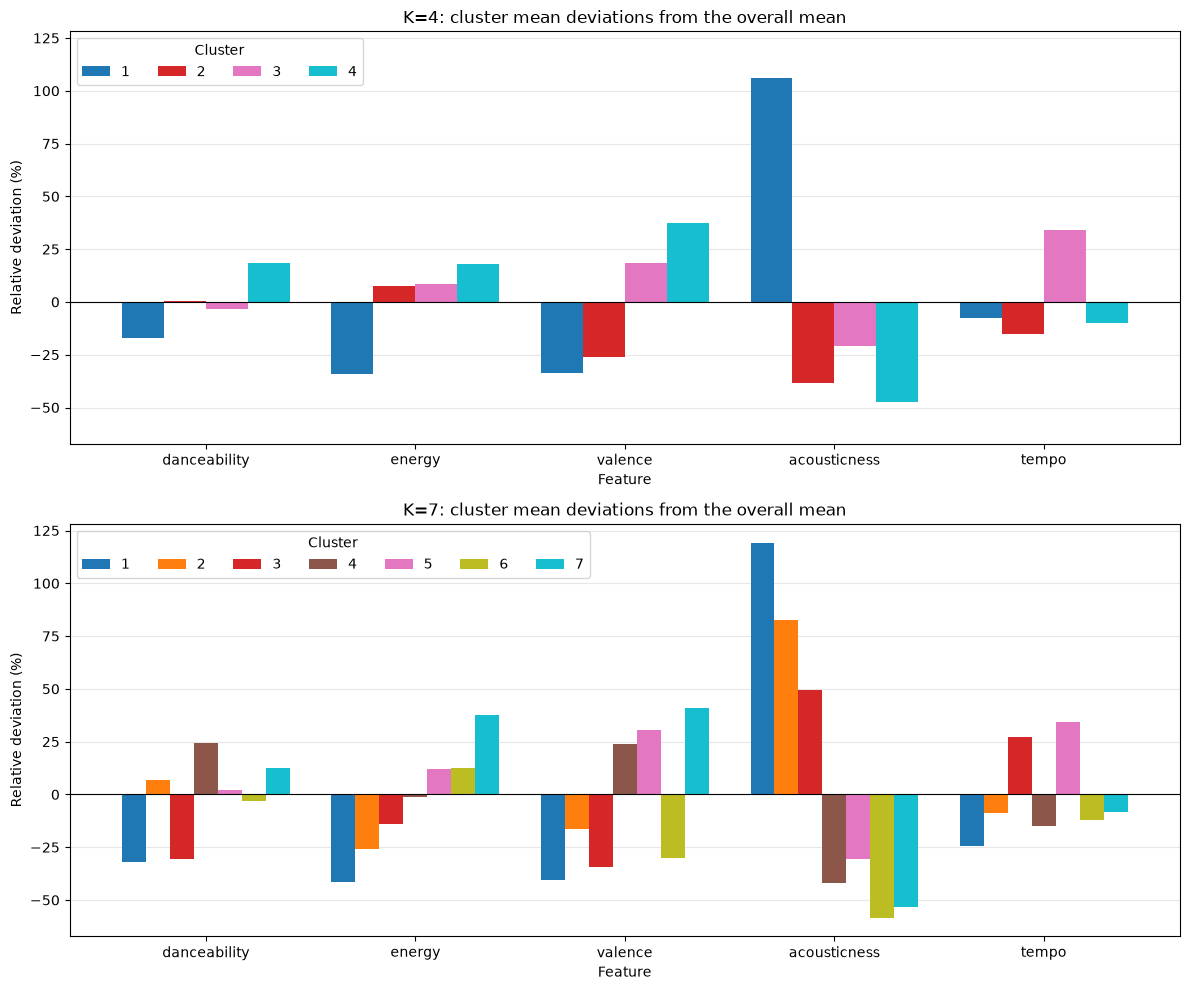
\includegraphics[width=0.85\textwidth]{a3_cluster_profiles.png}
  \caption{Cluster mean deviations from the overall mean (\%) for $K=4$ (top)
    and $K=7$ (bottom).}
  \label{fig:a3prof}
\end{figure}

\paragraph{Named interpretation of $K=4$}
(Table~\ref{tab:a3k4names}).

\begin{table}[H]
\centering
\caption{$K=4$: named interpretation of the clusters relative to the full
dataset.}
\label{tab:a3k4names}
\footnotesize
\begin{tabularx}{\textwidth}{@{}c r >{\raggedright\arraybackslash}X@{}}
\toprule
Cluster & Size / share & Interpretation \\
\midrule
1 & 253 / 25.3\,\% & \textbf{Mellow acoustic tracks:} acousticness
$+106.2\,\%$ (0.71 vs 0.34), energy $-34.1\,\%$, valence $-33.5\,\%$,
danceability $-17.3\,\%$; tempo slightly lower ($-7.7\,\%$). \\
2 & 235 / 23.5\,\% & \textbf{Energetic, electronic, darker-mood tracks:}
valence $-26.1\,\%$, acousticness $-38.3\,\%$, slower tempo ($-15.2\,\%$,
about 103 bpm); energy slightly above average ($+7.6\,\%$); danceability near
average ($+0.6\,\%$). \\
3 & 241 / 24.1\,\% & \textbf{Fast upbeat tracks:} tempo $+34.3\,\%$ (about
162 bpm), valence $+18.4\,\%$, acousticness $-20.6\,\%$, energy $+8.3\,\%$;
danceability near average ($-3.4\,\%$). \\
4 & 271 / 27.1\,\% & \textbf{Danceable, happy, energetic tracks:} valence
$+37.5\,\%$, danceability $+18.6\,\%$, energy $+17.9\,\%$, lowest
acousticness ($-47.5\,\%$); tempo slightly lower ($-10.1\,\%$). \\
\bottomrule
\end{tabularx}
\end{table}

\paragraph{Named interpretation of $K=7$}
(Table~\ref{tab:a3k7names}).

\begin{table}[H]
\centering
\caption{$K=7$: named interpretation of the clusters relative to the full
dataset.}
\label{tab:a3k7names}
\footnotesize
\begin{tabularx}{\textwidth}{@{}c r >{\raggedright\arraybackslash}X@{}}
\toprule
Cluster & Size / share & Interpretation \\
\midrule
1 & 102 / 10.2\,\% & \textbf{Slow, quiet, sad acoustic tracks:} acousticness
$+119.3\,\%$, energy $-41.5\,\%$, valence $-40.7\,\%$, danceability
$-32.0\,\%$, tempo $-24.4\,\%$ (about 91 bpm). \\
2 & 155 / 15.5\,\% & \textbf{Danceable acoustic-leaning tracks:} acousticness
$+82.7\,\%$, energy $-26.0\,\%$, valence $-16.5\,\%$; danceability slightly
above average ($+6.7\,\%$), tempo slightly lower ($-8.9\,\%$). \\
3 & 92 / 9.2\,\% & \textbf{Fast, non-danceable, dark semi-acoustic tracks:}
tempo $+27.2\,\%$ (about 154 bpm), danceability $-30.7\,\%$, valence
$-34.5\,\%$, acousticness $+49.2\,\%$, energy $-14.0\,\%$. \\
4 & 143 / 14.3\,\% & \textbf{Danceable, cheerful, electronic mid-tempo
tracks:} danceability $+24.2\,\%$, valence $+24.1\,\%$, acousticness
$-42.1\,\%$, tempo $-14.8\,\%$; energy near average ($-1.3\,\%$). \\
5 & 197 / 19.7\,\% & \textbf{Fast upbeat tracks:} tempo $+34.3\,\%$ (about
162 bpm), valence $+30.3\,\%$, energy $+12.1\,\%$, acousticness
$-30.8\,\%$; danceability near average ($+2.1\,\%$). \\
6 & 173 / 17.3\,\% & \textbf{Energetic, electronic, dark-mood tracks:}
acousticness $-58.4\,\%$, valence $-30.0\,\%$, energy $+12.7\,\%$, tempo
$-12.1\,\%$; danceability near average ($-3.2\,\%$). \\
7 & 138 / 13.8\,\% & \textbf{The most energetic and happiest tracks:} energy
$+37.4\,\%$, valence $+40.9\,\%$, danceability $+12.5\,\%$, acousticness
$-53.1\,\%$, tempo $-8.5\,\%$. \\
\bottomrule
\end{tabularx}
\end{table}

\begin{taskcomments}[Comments on Task~2]
\textbf{$K=4$} produces four clearly different profiles, each with two or
three dominant deviations (about $\pm30\,\%$ or more) that can be named
directly; the four clusters are of similar size (23.5--27.1\,\%).
\textbf{$K=7$} gives a more detailed partition (62.2\,\% of the scatter
explained against 50.1\,\%). Most $K=7$ clusters are refinements of the
$K=4$ clusters: $K=7$ clusters 1, 2 and 3 come mostly from $K=4$ cluster 1
(acoustic), cluster 5 corresponds to $K=4$ cluster 3 (fast upbeat), cluster 6
to $K=4$ cluster 2 (electronic, dark mood), and clusters 4 and 7 come mostly
from $K=4$ cluster 4 (danceable and happy). Several $K=7$ clusters differ
only in the strength of the same traits: clusters 4 and 7 are both danceable,
cheerful and electronic and differ mainly in energy ($-1.3\,\%$ vs
$+37.4\,\%$), and clusters 5 and 6 repeat the $K=4$ profiles almost
unchanged. Three clusters (1, 2, 3) split the acoustic group, with some
subtle differences, and several clusters are small (9.2--15.5\,\%).
\end{taskcomments}

\subsection{Task 3: judgement on which partition is better for interpretation}\label{sec:a3t3}

\textbf{$K=4$ is preferable for interpretation.} Although $K=7$ explains more
scatter (62.2\,\% vs 50.1\,\%)---as it must, since adding clusters can only
reduce the objective---its additional clusters largely re-split existing
profiles rather than revealing new ``types'', and three of its clusters
contain fewer than 16\,\% of the data. The $K=4$ partition has four
well-balanced clusters with distinct, directly nameable profiles, each of
which can be summarized in one sentence, which is exactly the level of detail
at which an interpretation remains robust.

\begin{taskcomments}[Comments on Task~3]
$K=7$ does give useful extra detail, mainly the split of the acoustic tracks
into slow and sad (cluster 1), danceable (cluster 2) and fast and dark
(cluster 3), but this makes the overall interpretation less concise. If a
finer analysis of the acoustic tracks is needed, $K=7$ is the better choice;
for a general description of the pop tracks, $K=4$ is enough. The judgement
therefore depends on the purpose, but for this assignment's question---which
partition is better \emph{for interpretation}---the answer is $K=4$.
\end{taskcomments}

% ==================================================================
\section{Assignment A4: contingency table}\label{sec:a4}

The assignment brief asks to (1) consider two nominal features, at most one
taken directly from the existing nominal features and the other developed by
the student; (2) build a contingency table, compute conditional frequency and
Quetelet index tables, and comment on the most strongly associated categories;
(3) compute and compare the average Quetelet index and Pearson's chi-squared;
(4) determine the numbers of observations sufficient to detect an association
at the 95\,\% and 99\,\% confidence levels, consulting statistical tables
online if necessary.

\subsection{Task 1: two nominal features}\label{sec:a4t1}

\begin{itemize}
  \item \textbf{\texttt{explicit}} is the existing nominal feature of the
        dataset: whether a track is marked as containing explicit lyrics
        (926 non-explicit, 74 explicit).
  \item \textbf{\texttt{popularity level}} is the feature developed for this
        assignment from the quantitative \texttt{popularity} score (0--100)
        with \texttt{pd.cut} on bins $[-1, 19, 69, 100]$: \textbf{low}
        (0--19), \textbf{medium} (20--69) and \textbf{high} (70--100). It
        yields three categories of similar size: 340, 343, and 317 tracks.
\end{itemize}

Before categorising, the popularity distribution was inspected
(Figure~\ref{fig:a4hist}): minimum 0, maximum 100, mean 47.58, median 66,
quartiles 2.0 / 66.0 / 71.0.

\begin{figure}[H]
  \centering
  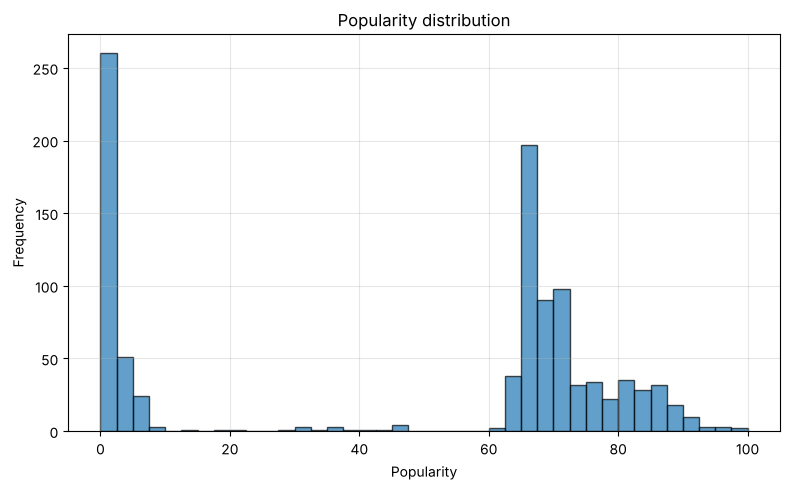
\includegraphics[width=0.62\textwidth]{a4_popularity_hist.png}
  \caption{Distribution of the popularity score in the pop subset: a large
    zero-score spike and a main mode around 70.}
  \label{fig:a4hist}
\end{figure}

The question behind the table: \emph{are explicit tracks distributed
differently over popularity levels than other tracks?}

\begin{taskcomments}[Comments on Task~1]
The cut points are round numbers chosen because \texttt{popularity} is
strongly bimodal: 338 tracks have a score below 20 (182 of them exactly 0),
and most of the others lie between 60 and 89. The mean-based categories of
the insurance example were deliberately not used: cut points based on the
mean (47.6) would produce categories with almost no observations, which
would make the chi-squared approximation unreliable. With the categories
above, all expected counts in the table are at least 23, so the chi-squared
approximation is valid.
\end{taskcomments}

\subsection{Task 2: contingency, conditional frequency, and Quetelet tables}\label{sec:a4t2}

\begin{table}[H]
\centering
\caption{Contingency table of popularity level and explicit flag (counts).}
\label{tab:a4cont}
\small
\begin{tabular}{lrrr}
\toprule
 & Non-explicit & Explicit & Total \\
\midrule
Low (0--19)    & 315 & 25 & 340 \\
Medium (20--69)& 338 & 5  & 343 \\
High (70--100) & 273 & 44 & 317 \\
\midrule
Total          & 926 & 74 & 1\,000 \\
\bottomrule
\end{tabular}
\end{table}

The marginal probabilities of the popularity levels are 0.340 (low), 0.343
(medium) and 0.317 (high). The conditional frequencies $P(x_1 \mid x_2)$
(column-normalized) and the Quetelet indices $q_{ij} = P(x_{1i}\mid
x_{2j})/P(x_{1i}) - 1$ are:

\begin{table}[H]
\centering
\caption{Conditional probabilities $P(\text{popularity level}\mid
\text{explicit})$ (top) and Quetelet indices (bottom).}
\label{tab:a4quetelet}
\small
\begin{tabular}{lrr}
\toprule
 & Non-explicit & Explicit \\
\midrule
\multicolumn{3}{l}{\textit{Conditional probabilities}} \\
Low    & 0.3402 & 0.3378 \\
Medium & 0.3650 & 0.0676 \\
High   & 0.2948 & 0.5946 \\
\midrule
\multicolumn{3}{l}{\textit{Quetelet indices}} \\
Low    & $+0.0005$ & $-0.0064$ \\
Medium & $+0.0642$ & $\mathbf{-0.8030}$ \\
High   & $-0.0700$ & $\mathbf{+0.8757}$ \\
\bottomrule
\end{tabular}
\end{table}

\begin{taskcomments}[Comments on Task~2]
The Quetelet index compares a conditional probability with the overall
proportion of the category: a positive value indicates a higher frequency, a
negative value a lower frequency, zero means the frequencies coincide, and
$-1$ means the cell is empty. The most strongly associated categories are the
two explicit-cell entries. \textbf{High popularity and explicit} ($q =
+0.8757$): high popularity occurs among 59.46\,\% of explicit tracks versus
31.70\,\% overall---about 1.88 times as often; among non-explicit tracks this
proportion is 29.48\,\%. \textbf{Medium popularity and explicit} ($q =
-0.8030$): only 6.76\,\% of explicit tracks (5 of 74) have a medium
popularity score, against 34.30\,\% overall---about 5 times less often. Low
popularity has a coefficient near zero for both groups ($-0.0064$ for
explicit, $+0.0005$ for non-explicit), so explicit tracks are as often
unpopular as the others: the difference is concentrated in the high and
medium levels. In other words, explicit tracks are rarely ``medium'' and are
over-represented among the hits. Within the non-explicit majority the
deviations from the marginals are small ($|q|\le 0.07$), because this group
is 92.6\,\% of the data and therefore close to the overall proportions. The
reverse conditional probability has a different meaning and should not be
confused with the forward one: among tracks with high popularity, 44 of 317
are explicit, or 13.88\,\%, compared with 7.40\,\% explicit tracks overall;
this is not the proportion of high popularity among explicit tracks
(59.46\,\%). Finally, the association says nothing about causes: it only
shows that explicit tracks in this sample are more often highly popular.
\end{taskcomments}

\subsection{Task 3: average Quetelet index versus Pearson chi-squared}\label{sec:a4t3}

The observation-weighted average Quetelet index is
\begin{equation}
  \bar{q} = \sum_{i,j} \frac{n_{ij}}{N}\,q_{ij} = 0.0371 .
\end{equation}
The weights are the cell proportions $n_{ij}/N$ (no absolute values; an
average over observations, not an unweighted average over cells). It
coincides, as expected, with $\chi^2/N$: Pearson $\chi^2 = 37.10$ with
$N = 1\,000$ and 2 degrees of freedom, so $\chi^2/N = 0.0371$ and
$\chi^2 = n \times \bar q$. The two numbers serve different purposes:
\begin{itemize}
  \item the \textbf{average Quetelet index} (0.0371) measures the
        \emph{strength} of the association and does not depend on the sample
        size: on average, knowing whether a track is explicit changes the
        probability of its popularity level by only about 3.7\,\%;
  \item \textbf{Pearson $\chi^2$} is the same quantity multiplied by $N$, so
        it grows with the sample size and is used to test \emph{whether} the
        association is significant: with 2 degrees of freedom the critical
        value is 5.99 at the 95\,\% level and 9.21 at the 99\,\% level, and
        the observed 37.10 is far above both ($p \approx 8.8\times10^{-9}$).
\end{itemize}

\begin{taskcomments}[Comments on Task~3]
The association is thus statistically very significant although its strength
is modest: the large cell-level coefficients (0.8757 and $-0.8030$) apply to
only 74 of 1\,000 observations and are weighted down in the average.
$\sqrt{\chi^2/N} = 0.193$ is Cram\'er's V for this table---a weak-to-moderate
association. As a robustness check on the independence assumption, 233 pop
tracks appear more than once in the file (listed on different albums), while
the $\chi^2$ test assumes independent observations; repeating the test with
only the 767 unique songs (same name and artist counted once) gives $\chi^2 =
33.28$, $\chi^2/n = 0.0434$, $p \approx 6\times10^{-8}$, so the conclusion
does not change.
\end{taskcomments}

\subsection{Task 4: sample sizes needed to detect the association}\label{sec:a4t4}

Keeping the proportions of Table~\ref{tab:a4cont} fixed, the required number
of observations follows from $\chi^2(N) = N\,\bar{q}$ scaling linearly:
\begin{equation}
  N_{\mathrm{req}} = N_{\mathrm{curr}} \cdot
  \frac{\chi^2_{\mathrm{critical}}}{\chi^2_{\mathrm{observed}}} ,
\end{equation}
Here $N_{\mathrm{curr}}$ is the contingency-table total and
$\chi^2_{\mathrm{observed}}$ is the test statistic, computed without Yates
correction. The degrees of freedom are $(R-1)\times(C-1) = 2$.
The critical values are the 95\,\% and 99\,\% chi-squared quantiles for two
degrees of freedom (computed with \texttt{chi2.ppf}), equivalent to consulting
a statistical table online. The smallest integer \emph{strictly
above} the boundary is selected as \texttt{floor($N_{\mathrm{req}}$)} $+ 1$,
so that the test statistic exceeds the critical value. The notebook's
step-by-step computation:
\begin{center}
\small
\begin{tabular}{llr}
\toprule
Step & Quantity & Value \\
\midrule
1 & $N_{\mathrm{curr}}$ (sum of all cells) & 1000 \\
2 & $\chi^2_{\mathrm{observed}}$ & 37.101995 \\
3 & dof $= (3-1)(2-1)$ & 2 \\
4 & $\chi^2_{\mathrm{crit}}$ at 95\,\% / 99\,\% & 5.991465 / 9.210340 \\
5 & $N_{\mathrm{req}}$ at 95\,\%: $1000 \cdot 5.991465 / 37.101995$ & 161.4863 \\
  & $N_{\mathrm{req}}$ at 99\,\%: $1000 \cdot 9.210340 / 37.101995$ & 248.2438 \\
6 & Minimum integer sample size & \textbf{162} / \textbf{249} \\
\bottomrule
\end{tabular}
\end{center}
The independence hypothesis would already be rejected at the 95\,\% level
with \textbf{162} observations (boundary 161.49), and at the 99\,\% level
with \textbf{249} (boundary 248.24), provided the proportions stay the same.
The present sample (1\,000 tracks) is far above both thresholds---only about
one sixth to one quarter of the data suffice, which agrees with the very
small $p$-value found above.

\begin{taskcomments}[Comments on Task~4]
This is a formal threshold based on the asymptotic chi-squared
approximation, not a power calculation or a guarantee for a new random
sample: the calculation assumes unchanged observed proportions, with $\chi^2$
growing proportionally to the sample size. A caution on small samples: with
about 162 observations and the same proportions there would be only about 12
explicit tracks, with expected cell counts of about 4 in each popularity
level, below the usual rule of 5, so the chi-squared approximation would be
rough there; at 249 observations the expected counts are about 6, which is
acceptable.
\end{taskcomments}

% ==================================================================
\section{Assignment A5: bootstrap confidence intervals}\label{sec:a5}

The assignment brief asks, for one K-means partition and one quantitative
feature, to (1) find a 95\,\% confidence interval for the mean over the full
dataset using bootstrap; (2) compare the feature means in two clusters using
bootstrap; (3) select the cluster whose mean is closest to the overall mean
and compare its mean with the overall mean using bootstrap---applying both
methods from the lecture \citep{efron,course}: \textbf{pivotal} (bootstrap
mean $\pm\,1.96$ bootstrap standard deviations) and \textbf{non-pivotal
(percentile)} (the 2.5th and 97.5th percentiles of the bootstrap
distribution), and interpreting the results.

\subsection{Setup: partition, feature, and procedure}\label{sec:a5setup}

The bootstrap analysis uses the \textbf{$K=4$ partition from Assignment~A3}
(features danceability, energy, valence, acousticness and tempo,
standardized; the best of 15 random starts, \texttt{random\_state}=3,
objective 2496.421---recomputing the partition reproduces exactly the same
labels) and the feature \texttt{energy}, by which the clusters are ordered.
Cluster means of energy are 0.3998, 0.6522, 0.6565, and 0.7150 in clusters
1--4 (sizes 253, 235, 241, 271), and the grand mean is 0.6064. All bootstrap
runs use \textbf{10\,000 resamples} of the 1\,000 observations drawn with
replacement (random generator \texttt{np.random.default\_rng(42)}), and both
lecture methods are applied to every task. Since \texttt{energy} is also one
of the clustering features, differences between clusters are partly built in
by the clustering itself; the tests below should be read with this in mind.

\subsection{Task 1: confidence interval for the grand mean}\label{sec:a5t1}

For each of the 10\,000 resamples the mean energy is computed; the pivotal
interval is the bootstrap mean $\pm\,1.96$ times the bootstrap standard
deviation (\texttt{std(ddof=1)}), and the percentile interval uses the 2.5th
and 97.5th percentiles:
\begin{center}
\small
\begin{tabular}{lcc}
\toprule
Original mean & Pivotal (95\,\%) & Non-pivotal / percentile (95\,\%) \\
\midrule
0.6064 & $[0.5956,\ 0.6173]$ & $[0.5957,\ 0.6171]$ \\
\bottomrule
\end{tabular}
\end{center}

\begin{figure}[H]
  \centering
  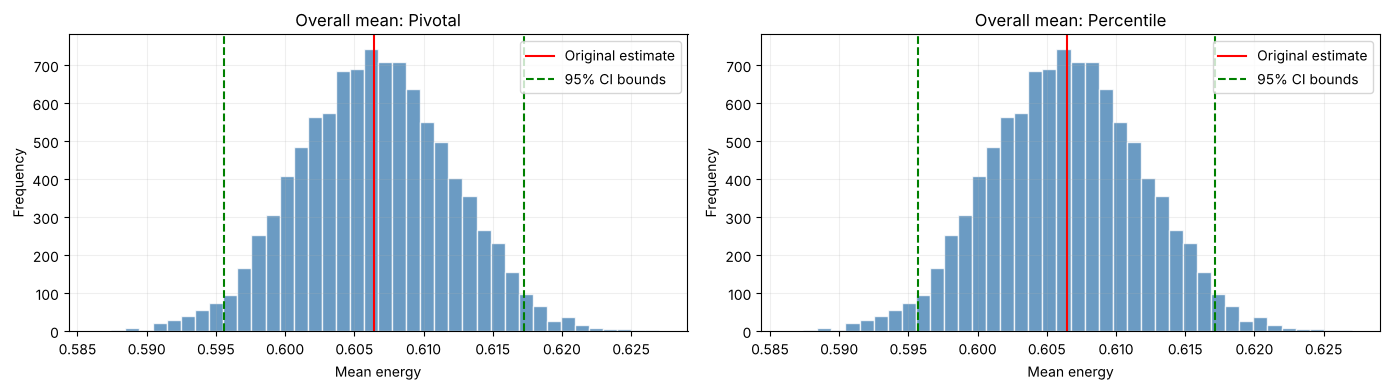
\includegraphics[width=0.95\textwidth]{a5_bootstrap_mean.png}
  \caption{Bootstrap distribution of the mean energy (10\,000 resamples) with
    the 95\,\% pivotal (left) and percentile (right) intervals; the red line
    marks the original estimate.}
  \label{fig:a5mean}
\end{figure}

\begin{taskcomments}[Comments on Task~1]
The two intervals are practically identical because the bootstrap
distribution of a mean of 1\,000 observations is almost symmetric and close
to normal (Figure~\ref{fig:a5mean}). The sample mean 0.6064 lies in the
middle of the interval, and the interval is narrow (width about 0.022): the
mean energy of pop tracks like these is estimated with a precision of about
$\pm0.011$. A caution: repeat listings of the same song are treated as
independent observations here, so the true uncertainty is slightly larger.
\end{taskcomments}

\subsection{Task 2: comparing two clusters}\label{sec:a5t2}

Clusters 2 and 3 are compared (sizes 235 and 241; means 0.6522 and 0.6565);
the observed difference is $0.6565 - 0.6522 = +0.0043$. Each resample redraws
1\,000 observations with their cluster labels, and the difference of the
within-cluster means of the resample is recorded:
\begin{center}
\small
\begin{tabular}{lcc}
\toprule
 & Pivotal & Percentile \\
\midrule
95\,\% CI for mean(3) $-$ mean(2) & $[-0.0176,\ 0.0263]$ & $[-0.0179,\ 0.0260]$ \\
\bottomrule
\end{tabular}
\end{center}

\begin{figure}[H]
  \centering
  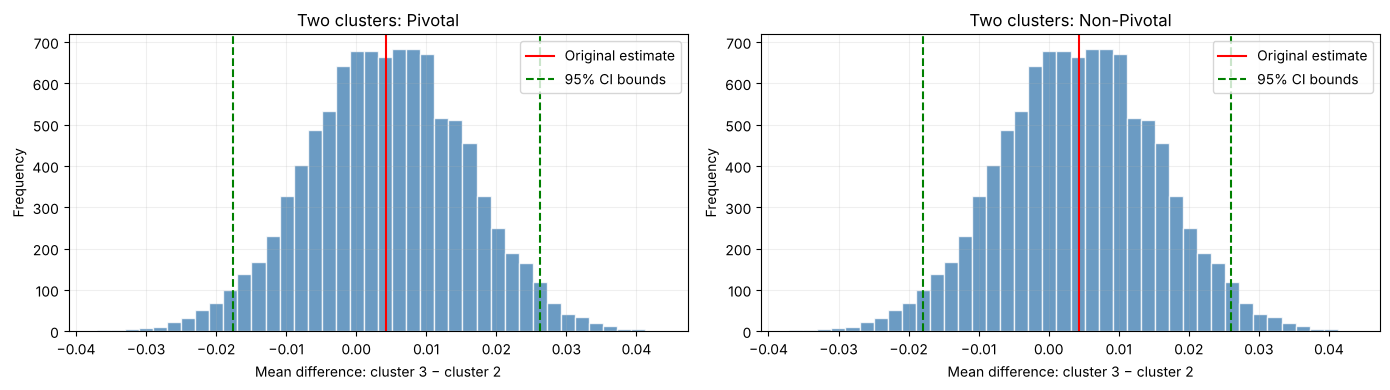
\includegraphics[width=0.95\textwidth]{a5_bootstrap_clusters.png}
  \caption{Bootstrap distribution of the difference between the mean energies
    of clusters 3 and 2 with the 95\,\% intervals.}
  \label{fig:a5clu}
\end{figure}

\begin{taskcomments}[Comments on Task~2]
Both intervals contain 0, so the hypothesis that the within-cluster means of
energy in clusters 2 and 3 are equal \textbf{cannot be rejected} (it is
accepted) at the 95\,\% confidence level: the observed difference (0.0043) is
five times smaller than the half-width of the intervals (about 0.022) and
cannot be distinguished from random variation. This agrees with the A3
interpretation, where both clusters had an energy about 8\,\% above the
average ($+7.6\,\%$ and $+8.3\,\%$): the clusters are separated by other
features (cluster 2 has a slow tempo and low valence, cluster 3 is fast and
cheerful), not by energy. A logical caution: failing to reject equality does
not prove that the means are exactly equal; it only shows that the data are
consistent with equality.
\end{taskcomments}

\subsection{Task 3: the nearest cluster versus the grand mean}\label{sec:a5t3}

The distances of the cluster means from the grand mean 0.6064 are:
\begin{center}
\small
\begin{tabular}{crrr}
\toprule
Cluster & Size & Mean energy & Distance \\
\midrule
1 & 253 & 0.3998 & 0.2066 \\
2 & 235 & 0.6522 & \textbf{0.0458} \\
3 & 241 & 0.6565 & 0.0501 \\
4 & 271 & 0.7150 & 0.1086 \\
\bottomrule
\end{tabular}
\end{center}
The cluster whose mean energy is closest to the grand mean is \textbf{cluster
2} (0.6522, difference $+0.0458$); cluster 3 is almost as close at $+0.0501$,
so the choice is a close call. Each resample yields
mean(within-cluster-2 part of the resample) $-$ mean(resample):
\begin{center}
\small
\begin{tabular}{lcc}
\toprule
 & Pivotal & Percentile \\
\midrule
95\,\% CI for cluster 2 $-$ grand mean & $[0.0297,\ 0.0620]$ & $[0.0298,\ 0.0617]$ \\
\bottomrule
\end{tabular}
\end{center}

\begin{figure}[H]
  \centering
  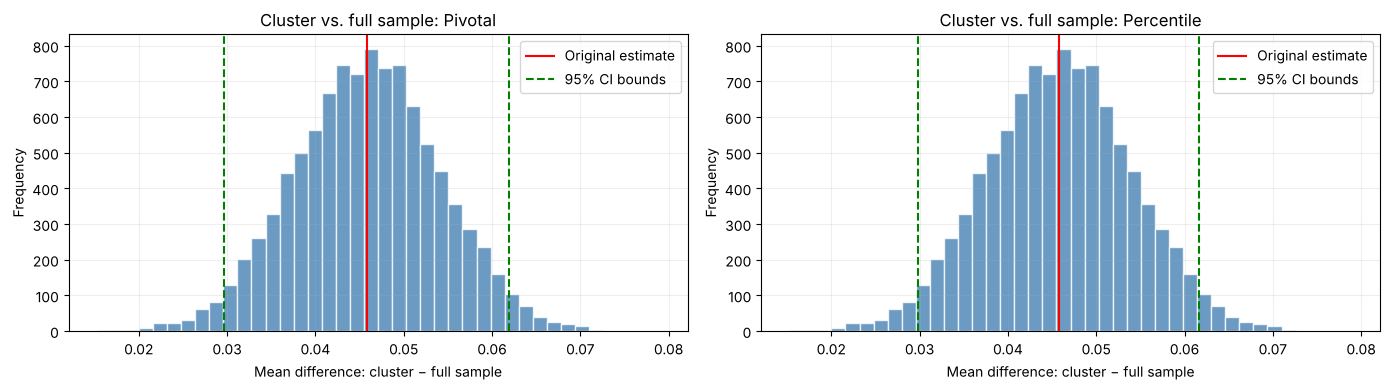
\includegraphics[width=0.95\textwidth]{a5_bootstrap_nearest.png}
  \caption{Bootstrap distribution of the difference between the mean energy of
    the nearest cluster (2) and the grand mean, with the 95\,\% intervals.}
  \label{fig:a5near}
\end{figure}

\begin{taskcomments}[Comments on Task~3]
Both intervals lie entirely above 0, so the hypothesis that the
within-cluster-2 mean coincides with the grand mean is \textbf{rejected} at
the 95\,\% level: even the cluster nearest to the grand mean has a mean
energy about 7.6\,\% higher than the overall mean, which is larger than the
random variation captured by the bootstrap. This differs from the insurance
example in the lecture materials, where the nearest cluster was consistent
with the grand mean. Two cautions accompany the conclusion: (i) the clusters
were built from the same data (and energy was one of the clustering
features), so such tests tend to find differences more easily than for
groups defined in advance; (ii) a cluster is part of the whole sample, so its
mean and the grand mean are not independent.
\end{taskcomments}

\subsection{Summary of the bootstrap results}\label{sec:a5sum}

Both versions of the bootstrap give the same conclusions in all three tasks
(Table~\ref{tab:a5sum}).

\begin{table}[H]
\centering
\caption{Summary of the bootstrap experiments (10\,000 resamples, 95\,\%
level).}
\label{tab:a5sum}
\small
\begin{tabular}{lcccc}
\toprule
Comparison & Observed & Pivotal CI & Percentile CI & Verdict \\
\midrule
Grand mean of energy            & 0.6064  & [0.5956, 0.6173]  & [0.5957, 0.6171]  & --- \\
Cluster 3 $-$ Cluster 2         & $+0.0043$ & $[-0.0176,\ 0.0263]$ & $[-0.0179,\ 0.0260]$ & not rejected \\
Cluster 2 $-$ grand mean        & $+0.0458$ & $[0.0297,\ 0.0620]$  & $[0.0298,\ 0.0617]$  & rejected \\
\bottomrule
\end{tabular}
\end{table}

% ==================================================================
\section{Discussion}\label{sec:disc}

\paragraph{A common least-squares thread.} The five assignments instantiate
the same principle at increasing complexity: A1 approximates a scatter cloud
by a line, A2 approximates a data matrix by a rank-2 (or rank-1) projection,
and A3 approximates it by $K$ centres---each time measuring quality by the
share of scatter explained ($\rho^2 = 52.3\,\%$; 65.5--67.6\,\% for two PCs
on the pop subset; 50.1--62.2\,\% for $K=4$/$K=7$). The lecture's warning
holds uniformly: a respectable explained
share does not guarantee precise individual predictions (A1: residual SD
1.77\,dB, and even the lecture's Iris example with $\rho^2 = 92.7\,\%$ leaves
20--32\,\% relative errors), and better objective values do not guarantee
better interpretations (A3: $K=7$ explains more but interprets worse).

\paragraph{Preprocessing is a modelling decision.} A2 shows that the PCA
answer depends on normalization: range normalization makes the observed span
of each feature equally important, z-scoring makes their standardized variances
equal, and the two solutions differ in loadings (e.g.\ loudness loses weight
under range normalization because its observed span is huge---8.97\,\% of the
range-normalized scatter against 20\,\% under z-scoring). The equivalence
of SVD with conventional correlation-matrix PCA on z-scored data (differences
of order $10^{-14}$--$10^{-15}$ on the pop subset) confirms that the
``preprocessing + SVD'' pipeline is not an
approximation \emph{to} PCA but \emph{is} PCA.

\paragraph{Association strength versus significance.} A4 illustrates the
lecture's distinction quantitatively: the popularity--explicit association is
highly significant ($p \approx 8.8\times10^{-9}$) yet modest in strength
($\bar q = 0.037$, Cram\'er's V $= 0.193$), because dramatic cell-level
Quetelet indices ($+0.876$, $-0.803$) concentrate in only 74 observations.
The same mechanism underlies the A5 bootstrap result: a difference can be
real (cluster 2 vs.\ grand mean, CI $[0.030,\ 0.062]$) or indistinguishable
from noise (cluster 3 vs.\ cluster 2, CI contains 0) depending on how many
observations carry it.

\paragraph{Stability and validation.} Three independent checks support the
robustness of the results: the A1 coefficients are unchanged on a seeded
hold-out split (test $R^2 = 0.5101$ vs.\ training 0.5228); the A4 conclusion
survives the removal of the 233 repeated listings ($\chi^2 = 33.28$ on 767
unique songs); and the K-means objective is stable across initializations
(six of fifteen $K=4$ runs within 0.25\,\% of the best).

\paragraph{Limitations.} (i) 233 pop tracks appear more than once (different
album listings), so observations are not perfectly independent; bootstrap
intervals and $\chi^2$ tests are therefore slightly optimistic. (ii) The pop
subset is a self-contained sample; conclusions need not transfer to other
genres. (iii) \texttt{energy} is both a
clustering feature (A3) and the compared feature (A5), so cluster differences
in energy are partly built in by construction. (iv) All findings are
descriptive associations, not causal effects.

% ==================================================================
\section{Conclusion}\label{sec:conc}

The five assignments solve one coherent analysis of 1\,000 pop tracks from
the Spotify Tracks dataset:

\begin{enumerate}
  \item \textbf{A1.} Loudness is linearly associated with energy
        ($\rho = 0.723$, $\rho^2 = 0.523$):
        $\mathrm{loudness} = -13.2765 + 10.4257\cdot\mathrm{energy}$, with
        MRAE of 23.13\,\% (DA) / 20.44\,\% (ML), residual SD 1.77\,dB and
        hold-out test $R^2 = 0.5101$---a solid tendency, imprecise per track.
  \item \textbf{A2.} Five audio features compress into two principal
        components holding 67.6\,\% (range) / 65.5\,\% (z-scored) of the
        scatter: an ``overall intensity'' PC1 and a tempo-vs-danceability
        PC2; SVD coincides with conventional PCA; the 74 explicit tracks
        shift mildly towards higher intensity; and a 0--100 hidden ranking
        factor of the ``energetic/upbeat'' aspect separates explicit (mean
        64.3) from non-explicit (mean 58.3) tracks.
  \item \textbf{A3.} K-means over danceability, energy, valence,
        acousticness and tempo yields four stable, nameable track types
        (mellow acoustic; energetic dark electronic; fast upbeat; danceable
        happy electronic); the finer $K=7$ partition explains more scatter
        but splits existing profiles, so $K=4$ is preferred for
        interpretation, while $K=7$ is the finer instrument when the acoustic
        group itself is of interest.
  \item \textbf{A4.} Popularity level and the explicit flag are significantly
        associated ($\chi^2 = 37.10$, $p\approx8.8\times10^{-9}$) with modest
        strength ($\bar q = 0.037$): explicit tracks reach high popularity
        1.9 times as often as average; 162/249 observations suffice to detect
        the association at the 95/99\,\% levels, and the conclusion survives
        the unique-song robustness check.
  \item \textbf{A5.} The mean energy of pop tracks is $0.606 \pm 0.011$
        (95\,\%); clusters 2 and 3 are indistinguishable in energy, while
        even the cluster nearest to the grand mean differs from it
        significantly ($+0.046$, CI $[0.030,\ 0.062]$).
\end{enumerate}

Beyond the specific numbers, the project demonstrates the course's central
message: regression, PCA, and clustering are one family of least-squares
approximation methods; preprocessing and granularity are modelling decisions
that change both objective values and interpretations; and statistical
significance, association strength, and prediction precision are three
different questions that must be answered separately.

% ==================================================================
\phantomsection
\addcontentsline{toc}{section}{References}

\begin{thebibliography}{9}

\bibitem[Galton(1886)]{galton}
Galton, F. (1886).
\newblock Regression towards mediocrity in hereditary stature.
\newblock \textit{Journal of the Anthropological Institute}, 15, 246--263.

\bibitem[Pearson(1895)]{pearson}
Pearson, K. (1895).
\newblock Notes on regression and inheritance in the case of two parents.
\newblock \textit{Proceedings of the Royal Society of London}, 58, 240--242.

\bibitem[Kaggle(2020--2024)]{spotify}
Kaggle (2020--2024).
\newblock \textit{Spotify Tracks Dataset (114k songs)}.
\newblock \url{https://www.kaggle.com/datasets/maharshipandya/spotify-tracks-dataset}

\bibitem[Mirkin(2026)]{lecture}
Mirkin, B. (2026).
\newblock \textit{Basics of Data Analysis. Lecture 2: 2D Regression and
  Correlation Coefficient}.
\newblock HSE University, lecture notes.

\bibitem[Mirkin(2026b)]{lecture3}
Mirkin, B. (2026).
\newblock \textit{Basics of Data Analysis. Lecture 3: Principal Component
  Analysis and SVD}.
\newblock HSE University, lecture notes.

\bibitem[Mirkin(2026c)]{course}
Mirkin, B. (2026).
\newblock \textit{Basics of Data Analysis: course materials and homework
  assignment briefs (K-means clustering, contingency tables, bootstrap)}.
\newblock HSE University, lecture notes.

\bibitem[MacQueen(1967)]{macqueen}
MacQueen, J. (1967).
\newblock Some methods for classification and analysis of multivariate
  observations.
\newblock \textit{Proceedings of the Fifth Berkeley Symposium on Mathematical
  Statistics and Probability}, 1, 281--297.

\bibitem[Efron(1979)]{efron}
Efron, B. (1979).
\newblock Bootstrap methods: another look at the jackknife.
\newblock \textit{The Annals of Statistics}, 7(1), 1--26.

\end{thebibliography}

\end{document}
